\documentclass[thesis]{subfiles}

\begin{document}

\OnlyInSubfile{\setcounter{chapter}{4}}
\chapter{Classical simulations}

\TODO: general intro

\newpage
\section{Intrusion of electrolyte in ZIF-8}

One of the novel applications that has been proposed for hydrophobic nanoporous
materials is related to mechanical energy storage or dissipation through water
intrusion\cite{Eroshenko2001, Soulard2004}. In a hydrophobic porous material,
the pressure at which external water will enter the pore space is greater than
the vapor pressure of water. That is, adsorption happens only in the liquid
phase --- and this high-pressure adsorption is called
\emph{intrusion}\cite{Fraux2017}. This phenomenon has been extensively studied
in inorganic nanoporous materials, such as zeolites\cite{Saada2010,
Desbiens2005, Humplik2014a, Humplik2014b}, and more recently evidenced in
hydrophobic metal--organic frameworks\cite{Ortiz2013, Grosu2015,
MichelinJamois2015}. Depending on the nature of the nanoporous material and the
strength of the host--guest interactions, intrusion curves can have different
shapes and be classified as either as a molecular spring, a shock adsorber, or a
bumper. This classification depends on the level of hysteresis during an
intrusion--extrusion cycle.

A very sought-after property related to the intrusion of water in hydrophobic
frameworks is the ability to tune the intrusion pressure and the amount of
hysteresis present. This can be achieved by chemical modifications of the
structure of the host material\cite{AOrtiz2014}, or by changing the nature of
the liquid --- namely, by adding ions to the water\cite{Ortiz2014}. Depending on
the size of the ions and porous channels, in some cases only water can enter the
nanopores while ions stay in the bulk liquid. The change in the intrusion
pressure is then directly related to additional osmotic pressure the fluid has
to overcome to enter the structure\cite{MichelinJamois2015}. But in other cases,
the addition of ions has a more complex impact on both the intrusion pressure
and the shape of intrusion curves. For example, in the pure-silica analogue of
the $\beta$ zeolite\cite{Camblor1996}, increasing the electrolyte concentration
from \SI{5}{mol/L} to \SI{10}{mol/L} only shifts the intrusion pressure, but
increasing it again to \SI{15}{mol/L} changes the overall behavior from a
shock-absorber to a spring\cite{Ryzhikov2014}. Such changes indicate that the
interaction between the electrolyte fluid and the host structure is not merely
reduced to a simple effect of size-based exclusion. At the same time, \emph{in
situ} X-ray diffraction measurements performed during intrusion--extrusion
cycles showed that \ce{MgCl2} ions can enter a pure-silica ferrierite during
intrusion\cite{Arletti2016}. All this evidence points to a more complex effect
than pure osmotic pressure when using an electrolyte fluid for intrusion.

Moreover, we know that adsorption of water in the gas phase can induce large
structural changes in nanoporous materials\cite{Lee2001, Seoung2013}. This is
particular true of soft porous crystals\cite{Horike2009}, such as
flexible MOFs\cite{Schneemann2014}, exhibiting dynamic frameworks that are
able to respond to external stimuli. This has been studied, by both experimental
and computational means, on the MIL-53 family of "breathing" frameworks: the
presence of water influences the structure of MIL-53(Cr)\cite{Haigis2013}, and
is responsible for the occurrence of numerous structural transitions in
MIL-53(Ga), as a function of both water vapor pressure and
temperature\cite{Boutin2013, Coudert2014}. Relatively little is known, in
contrast, on the impact of liquid water --- and aqueous solution --- intrusion
on the structure of flexible MOFs.

Here, we are interested in the study of the high-pressure electrolyte intrusion
in \ZIF8. \ZIF8 is hydrophobic\cite{AOrtiz2014}, and presents interesting
behavior upon intrusion. While osmotic pressure effects do not depend on the
chemical nature of the ions, \ZIF8 shows changes from one energetic behavior to
another when the ion nature changes while keeping concentration
constant\cite{Ortiz2014}. \ZIF8 behavior can also be tuned chemically, by
modifying the nature of the linkers, for example changing the methylimidazolate
to a chloroimidazolate increases the intrusion pressure\cite{Mortada2018}.

However, the exact mechanism and behavior at the molecular level upon intrusion
of electrolytes in \ZIF8 are still unknown. In this work, I used classical
molecular simulations to study the structure, dynamics and energetic
implications of confining water and aqueous solutions of LiCl in \ZIF8. Using
these simulations, I was able to explore different aspects of the \{water,
\ZIF8\} and \{electrolyte, \ZIF8\} systems. I describe below the structure of
the liquids and the influence of confinement, their dynamics, the mechanical
properties of \ZIF8 and the impact of liquid intrusion on them. We conclude by a
series of considerations on the energetic behavior of intrusion, and results on
the thermodynamics and the free energy of entry of ions in \ZIF8.

\subsubsection{Computational methods}

We ran classical molecular dynamics (MD) simulations and umbrella sampling
simulations using the LAMMPS\cite{Plimpton1993} code. The umbrella sampling
simulations additionally used the COLVARS\cite{Fiorin2013} module for collective
variables. We used a combination of different force fields for the component of
the system: a rigid SPC/E\cite{Berendsen1987} for water, for its ability to
describe the dynamics of liquid water and the solvation of ions; a flexible
force-field adapted from AMBER by \citeauthor{Zheng2012}\cite{Zheng2012} for the
description of the \ZIF8 framework; and a combination of electrostatic and
Lennard-Jones potentials for the ions\cite{Chowdhuri2003}. We used
Lorentz-Berthelot mixing rules for cross-terms in Lennard-Jones potential, and
Ewald summation to account efficiently for electrostatic interactions. We used a
cutoff of \SI{8.5}{\angstrom} for both the Lennard-Jones potential and the
separation between real space and Fourier space in the Ewald summation.

After an initial energy minimization, we carried all simulations in the
isothermal-isobaric $(N, P, T)$ ensemble with a timestep of \SI{1}{fs}, using a
Nosé-Hoover thermostat with a time constant of \SI{1}{ps} and a Nosé-Hoover
barostat with a time constant of \SI{10}{ps}. We allowed the barostat to make
arbitrary changes to unit cell lengths and tilt factors (fully flexible
anisotropic cell), while imposing an isotropic pressure to the system. Unless
specified otherwise, we ran all simulations in the $(N, P, T)$ ensemble for
\SI{10}{ns}, and only used the last \SI{4}{ns} for analysis.

We used three different types of systems in this study. First, bulk liquids at
different LiCl concentration: \SI{0}{mol/L} (pure water), \SI{1}{mol/L},
\SI{5}{mol/L}, \SI{10}{mol/L}, \SI{15}{mol/L} and \SI{20}{mol/L} --- the
experimental solubility of LiCl in water at 25~{\textdegree C} is
\SI{19.87}{mol/L}. Then we simulated a $3\times3\times3$ super-cell of \ZIF8,
with liquid confined inside the pores, at the same concentrations as the bulk
liquid. Finally, we used a $2\times2\times3$ \ZIF8 super-cell containing pure
water together with a \SI{34}{\angstrom} cubic reservoir of water on top (this
system featuring an explicit \ZIF8/liquid interface) for the umbrella sampling
simulations.

We generated the initial configuration using the packmol
software\cite{Martnez2009}, randomly placing the desired number of particles in
the system. We started with bulk electrolyte in a \SI{32}{\angstrom} cubic box
containing 750 water molecules for the pure water, and added ions for the
different LiCl concentrations. For the liquids confined in \ZIF8, we needed to
know how many molecules would fit in the \ZIF8 pores. For that, we ran a
constant pressure simulation with a reservoir of pure water outside an empty
$2\times2\times3$ \ZIF8 super-cell at \SI{0.5}{GPa}. We ran the simulation for
\SI{10}{ns} and counted, and counted 75 water molecules in one unit cell. We
then ran simulations of the bulk liquid at varying concentration at the constant
pressure of \SI{0}{GPa}, and recorded the corresponding particles density. Using
the density of pure water, we mapped the 75 molecules per unit cell to an
accessible porous volume of \SI{2.286}{nm^3}, or {46\%} of the unit cell. From
this volume and the density of the bulk liquids, we could now compute the number
of molecule to put in the $3\times3\times3$ super-cell for each concentration.
The resulting system was a cubic box of \SI{51}{\angstrom}, containing roughly
13\,000 atoms.

\subsection{Structuration of the liquid}
\label{sec:liquid-structure}

From the point of view of the liquid, the principal effect of intrusion is the
confinement of the fluid to a pore space of nanometric dimensions, i.e. the
nanoporous material acts as a host matrix --- although a flexible one. Here, we
look at the effects of this confinement on the liquid structure, as a function
of the electrolyte concentration. In order to characterize the structure of the
liquid and the solvation of ions confined in \ZIF8, we computed radial
distribution function for each pair of atom types in the system. Integrating the
radial distribution function until the first minimum gives the number of
neighbors in the first solvation shell of each atom. The evolution of this
number of neighbors as a function of LiCl concentration is presented in
figure~\ref{fig:licl-zif:neighbors}, for both the bulk liquid and the confined
liquid.

\begin{figure}[ht]
    \centering
    % GNUPLOT: LaTeX picture with Postscript
\begingroup
  \makeatletter
  \providecommand\color[2][]{%
    \GenericError{(gnuplot) \space\space\space\@spaces}{%
      Package color not loaded in conjunction with
      terminal option `colourtext'%
    }{See the gnuplot documentation for explanation.%
    }{Either use 'blacktext' in gnuplot or load the package
      color.sty in LaTeX.}%
    \renewcommand\color[2][]{}%
  }%
  \providecommand\includegraphics[2][]{%
    \GenericError{(gnuplot) \space\space\space\@spaces}{%
      Package graphicx or graphics not loaded%
    }{See the gnuplot documentation for explanation.%
    }{The gnuplot epslatex terminal needs graphicx.sty or graphics.sty.}%
    \renewcommand\includegraphics[2][]{}%
  }%
  \providecommand\rotatebox[2]{#2}%
  \@ifundefined{ifGPcolor}{%
    \newif\ifGPcolor
    \GPcolortrue
  }{}%
  \@ifundefined{ifGPblacktext}{%
    \newif\ifGPblacktext
    \GPblacktextfalse
  }{}%
  % define a \g@addto@macro without @ in the name:
  \let\gplgaddtomacro\g@addto@macro
  % define empty templates for all commands taking text:
  \gdef\gplbacktext{}%
  \gdef\gplfronttext{}%
  \makeatother
  \ifGPblacktext
    % no textcolor at all
    \def\colorrgb#1{}%
    \def\colorgray#1{}%
  \else
    % gray or color?
    \ifGPcolor
      \def\colorrgb#1{\color[rgb]{#1}}%
      \def\colorgray#1{\color[gray]{#1}}%
      \expandafter\def\csname LTw\endcsname{\color{white}}%
      \expandafter\def\csname LTb\endcsname{\color{black}}%
      \expandafter\def\csname LTa\endcsname{\color{black}}%
      \expandafter\def\csname LT0\endcsname{\color[rgb]{1,0,0}}%
      \expandafter\def\csname LT1\endcsname{\color[rgb]{0,1,0}}%
      \expandafter\def\csname LT2\endcsname{\color[rgb]{0,0,1}}%
      \expandafter\def\csname LT3\endcsname{\color[rgb]{1,0,1}}%
      \expandafter\def\csname LT4\endcsname{\color[rgb]{0,1,1}}%
      \expandafter\def\csname LT5\endcsname{\color[rgb]{1,1,0}}%
      \expandafter\def\csname LT6\endcsname{\color[rgb]{0,0,0}}%
      \expandafter\def\csname LT7\endcsname{\color[rgb]{1,0.3,0}}%
      \expandafter\def\csname LT8\endcsname{\color[rgb]{0.5,0.5,0.5}}%
    \else
      % gray
      \def\colorrgb#1{\color{black}}%
      \def\colorgray#1{\color[gray]{#1}}%
      \expandafter\def\csname LTw\endcsname{\color{white}}%
      \expandafter\def\csname LTb\endcsname{\color{black}}%
      \expandafter\def\csname LTa\endcsname{\color{black}}%
      \expandafter\def\csname LT0\endcsname{\color{black}}%
      \expandafter\def\csname LT1\endcsname{\color{black}}%
      \expandafter\def\csname LT2\endcsname{\color{black}}%
      \expandafter\def\csname LT3\endcsname{\color{black}}%
      \expandafter\def\csname LT4\endcsname{\color{black}}%
      \expandafter\def\csname LT5\endcsname{\color{black}}%
      \expandafter\def\csname LT6\endcsname{\color{black}}%
      \expandafter\def\csname LT7\endcsname{\color{black}}%
      \expandafter\def\csname LT8\endcsname{\color{black}}%
    \fi
  \fi
    \setlength{\unitlength}{0.0500bp}%
    \ifx\gptboxheight\undefined%
      \newlength{\gptboxheight}%
      \newlength{\gptboxwidth}%
      \newsavebox{\gptboxtext}%
    \fi%
    \setlength{\fboxrule}{0.5pt}%
    \setlength{\fboxsep}{1pt}%
\begin{picture}(6800.00,3960.00)%
    \gplgaddtomacro\gplbacktext{%
      \csname LTb\endcsname%%
      \put(514,694){\makebox(0,0)[r]{\strut{}$0$}}%
      \csname LTb\endcsname%%
      \put(514,1456){\makebox(0,0)[r]{\strut{}$2$}}%
      \csname LTb\endcsname%%
      \put(514,2218){\makebox(0,0)[r]{\strut{}$4$}}%
      \csname LTb\endcsname%%
      \put(514,2980){\makebox(0,0)[r]{\strut{}$6$}}%
      \csname LTb\endcsname%%
      \put(514,3742){\makebox(0,0)[r]{\strut{}$8$}}%
      \csname LTb\endcsname%%
      \put(633,477){\makebox(0,0){\strut{}$0$}}%
      \csname LTb\endcsname%%
      \put(1996,477){\makebox(0,0){\strut{}$5$}}%
      \csname LTb\endcsname%%
      \put(3359,477){\makebox(0,0){\strut{}$10$}}%
      \csname LTb\endcsname%%
      \put(4722,477){\makebox(0,0){\strut{}$15$}}%
      \csname LTb\endcsname%%
      \put(6085,477){\makebox(0,0){\strut{}$20$}}%
      \csname LTb\endcsname%%
      \put(6204,694){\makebox(0,0)[l]{\strut{}$0$}}%
      \csname LTb\endcsname%%
      \put(6204,1456){\makebox(0,0)[l]{\strut{}$2$}}%
      \csname LTb\endcsname%%
      \put(6204,2218){\makebox(0,0)[l]{\strut{}$4$}}%
      \csname LTb\endcsname%%
      \put(6204,2980){\makebox(0,0)[l]{\strut{}$6$}}%
      \csname LTb\endcsname%%
      \put(6204,3742){\makebox(0,0)[l]{\strut{}$8$}}%
      \csname LTb\endcsname%%
      \put(3168,3171){\makebox(0,0)[l]{\strut{}Li-Cl neighbors}}%
    }%
    \gplgaddtomacro\gplfronttext{%
      \csname LTb\endcsname%%
      \put(178,2218){\rotatebox{-270}{\makebox(0,0){\strut{}Water neighbors}}}%
      \csname LTb\endcsname%%
      \put(3359,152){\makebox(0,0){\strut{}Concentration (mol/L)}}%
      \csname LTb\endcsname%%
      \put(2218,3547){\makebox(0,0)[r]{\strut{}water}}%
      \csname LTb\endcsname%%
      \put(3375,3547){\makebox(0,0)[r]{\strut{}Li}}%
      \csname LTb\endcsname%%
      \put(4532,3547){\makebox(0,0)[r]{\strut{}Cl}}%
    }%
    \gplbacktext
    \put(0,0){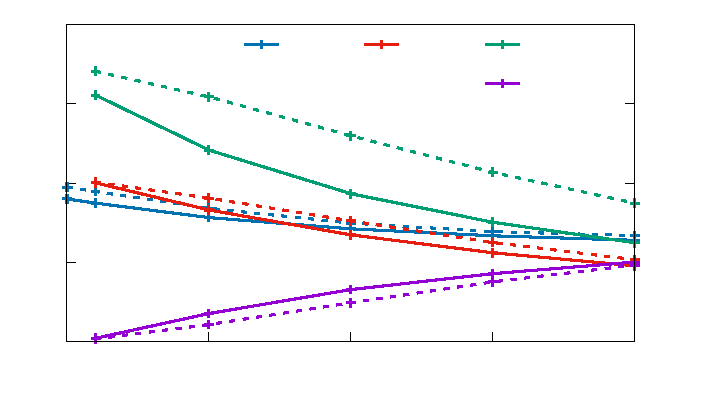
\includegraphics{licl-zif-neighbors}}%
    \gplfronttext
  \end{picture}%
\endgroup

    \caption{Number of water neighbors in the first solvation shell in the
    confined liquid (plain lines) and the bulk liquid (dotted lines) as
    function of the concentration, at the constant pressure of \SI{0}{GPa}.
    The number of chlorine neighbors for lithium ions is also represented.}
    \label{fig:licl-zif:neighbors}
\end{figure}

The first thing we can see here is that, for all species (Li, Cl and water), the
number of neighboring water molecules --- i.e., the solvation --- decreases as
the LiCl concentration increases. At \SI{0}{mol/L} and \SI{1}{mol/L}, there are
more than enough water molecules with respect to the ions (roughly 55 water
molecule per ion at \SI{1}{mol/L}) so that they can be in their ideal solvation
state: 4 \ce{H2O} per \ce{Li+}, and 6 \ce{H2O} per \ce{Cl-}. But as the
concentration increases, there are fewer available water molecules and the ions
have to accommodate by having less molecule in their first solvation shell. At
\SI{20}{mol/L}, there are only 2.7 water molecule available for each lithium
ion; and each cation is thus surrounded by 1.9 water molecule, less than half
its complete solvation state. The same is true for water/water coordination
through hydrogen bonds, as the water molecules compete with the ions to surround
themselves with other water molecules.

In the bulk liquid, the loss of neighbors is linear with the concentration, as
all the molecules in the system are able to adapt to find the state of largest
possible solvation. In the confined liquid however, the molecules are
geometrically constrained by the presence of the \ZIF8 framework, which
manifests as an excluded volume, and thus are not able to adapt as well to the
increase in LiCl concentration, making the number of neighbors drop faster. We
also note a slight increase in the number of chlorine neighbors of lithium ions
at intermediate concentration, compared to the bulk: the effect of confinement,
by diminishing the solvation of the ions, favors the occurrence of anion--cation
pairs. The number of lithium neighbors for chlorine ions is the same as the
number of chlorine neighbors for lithium ions.

Going from bulk liquid to confined liquid also changes the number of neighbors
for water and Cl ions, even at \SI{1}{mol/L}. In addition to preventing a full
reorganization of the water molecules when the concentration increases, the
presence of the framework also affects the structure of the solvation shells.
Molecules close to the framework can only have neighbors from the liquid on one
side --- an excluded volume effect. However, the framework also has an effect at
longer range, the available space in the pores dictating the arrangement of
molecules. Instead of being widely distributed, the molecules are restricted to
specific preferential locations, due to host--guest interactions. This effect is
particularly visible on figure~\ref{fig:licl-zif:density}, and is stronger on Cl/water
pairs than water/water or Li/water, as the Cl has a larger radius and binds to
the hydrogen atoms in water, making its solvation sphere both bigger and
"softer".

\begin{figure}[ht]
    \centering
    % GNUPLOT: LaTeX picture with Postscript
\begingroup
  \makeatletter
  \providecommand\color[2][]{%
    \GenericError{(gnuplot) \space\space\space\@spaces}{%
      Package color not loaded in conjunction with
      terminal option `colourtext'%
    }{See the gnuplot documentation for explanation.%
    }{Either use 'blacktext' in gnuplot or load the package
      color.sty in LaTeX.}%
    \renewcommand\color[2][]{}%
  }%
  \providecommand\includegraphics[2][]{%
    \GenericError{(gnuplot) \space\space\space\@spaces}{%
      Package graphicx or graphics not loaded%
    }{See the gnuplot documentation for explanation.%
    }{The gnuplot epslatex terminal needs graphicx.sty or graphics.sty.}%
    \renewcommand\includegraphics[2][]{}%
  }%
  \providecommand\rotatebox[2]{#2}%
  \@ifundefined{ifGPcolor}{%
    \newif\ifGPcolor
    \GPcolortrue
  }{}%
  \@ifundefined{ifGPblacktext}{%
    \newif\ifGPblacktext
    \GPblacktextfalse
  }{}%
  % define a \g@addto@macro without @ in the name:
  \let\gplgaddtomacro\g@addto@macro
  % define empty templates for all commands taking text:
  \gdef\gplbacktext{}%
  \gdef\gplfronttext{}%
  \makeatother
  \ifGPblacktext
    % no textcolor at all
    \def\colorrgb#1{}%
    \def\colorgray#1{}%
  \else
    % gray or color?
    \ifGPcolor
      \def\colorrgb#1{\color[rgb]{#1}}%
      \def\colorgray#1{\color[gray]{#1}}%
      \expandafter\def\csname LTw\endcsname{\color{white}}%
      \expandafter\def\csname LTb\endcsname{\color{black}}%
      \expandafter\def\csname LTa\endcsname{\color{black}}%
      \expandafter\def\csname LT0\endcsname{\color[rgb]{1,0,0}}%
      \expandafter\def\csname LT1\endcsname{\color[rgb]{0,1,0}}%
      \expandafter\def\csname LT2\endcsname{\color[rgb]{0,0,1}}%
      \expandafter\def\csname LT3\endcsname{\color[rgb]{1,0,1}}%
      \expandafter\def\csname LT4\endcsname{\color[rgb]{0,1,1}}%
      \expandafter\def\csname LT5\endcsname{\color[rgb]{1,1,0}}%
      \expandafter\def\csname LT6\endcsname{\color[rgb]{0,0,0}}%
      \expandafter\def\csname LT7\endcsname{\color[rgb]{1,0.3,0}}%
      \expandafter\def\csname LT8\endcsname{\color[rgb]{0.5,0.5,0.5}}%
    \else
      % gray
      \def\colorrgb#1{\color{black}}%
      \def\colorgray#1{\color[gray]{#1}}%
      \expandafter\def\csname LTw\endcsname{\color{white}}%
      \expandafter\def\csname LTb\endcsname{\color{black}}%
      \expandafter\def\csname LTa\endcsname{\color{black}}%
      \expandafter\def\csname LT0\endcsname{\color{black}}%
      \expandafter\def\csname LT1\endcsname{\color{black}}%
      \expandafter\def\csname LT2\endcsname{\color{black}}%
      \expandafter\def\csname LT3\endcsname{\color{black}}%
      \expandafter\def\csname LT4\endcsname{\color{black}}%
      \expandafter\def\csname LT5\endcsname{\color{black}}%
      \expandafter\def\csname LT6\endcsname{\color{black}}%
      \expandafter\def\csname LT7\endcsname{\color{black}}%
      \expandafter\def\csname LT8\endcsname{\color{black}}%
    \fi
  \fi
    \setlength{\unitlength}{0.0500bp}%
    \ifx\gptboxheight\undefined%
      \newlength{\gptboxheight}%
      \newlength{\gptboxwidth}%
      \newsavebox{\gptboxtext}%
    \fi%
    \setlength{\fboxrule}{0.5pt}%
    \setlength{\fboxsep}{1pt}%
\begin{picture}(7360.00,7080.00)%
    \gplgaddtomacro\gplbacktext{%
      \csname LTb\endcsname%%
      \put(578,5032){\makebox(0,0)[r]{\strut{}\tiny -0.5}}%
      \csname LTb\endcsname%%
      \put(578,5482){\makebox(0,0)[r]{\strut{}\tiny -0.25}}%
      \csname LTb\endcsname%%
      \put(578,5932){\makebox(0,0)[r]{\strut{}\tiny 0}}%
      \csname LTb\endcsname%%
      \put(578,6382){\makebox(0,0)[r]{\strut{}\tiny 0.25}}%
      \csname LTb\endcsname%%
      \put(578,6832){\makebox(0,0)[r]{\strut{}\tiny 0.5}}%
      \csname LTb\endcsname%%
      \put(646,4908){\makebox(0,0){\strut{}\tiny -0.5}}%
      \csname LTb\endcsname%%
      \put(1096,4908){\makebox(0,0){\strut{}\tiny -0.25}}%
      \csname LTb\endcsname%%
      \put(1546,4908){\makebox(0,0){\strut{}\tiny 0}}%
      \csname LTb\endcsname%%
      \put(1995,4908){\makebox(0,0){\strut{}\tiny 0.25}}%
      \csname LTb\endcsname%%
      \put(2445,4908){\makebox(0,0){\strut{}\tiny 0.5}}%
      \colorrgb{1.00,0.00,0.00}%%
      \put(74,5899){\makebox(0,0)[l]{\strut{}O}}%
      \colorrgb{0.00,0.00,1.00}%%
      \put(74,3681){\makebox(0,0)[l]{\strut{}Li}}%
      \colorrgb{0.00,0.32,0.19}%%
      \put(74,1321){\makebox(0,0)[l]{\strut{}Cl}}%
    }%
    \gplgaddtomacro\gplfronttext{%
      \csname LTb\endcsname%%
      \put(1545,7018){\makebox(0,0){\strut{}1 mol/L}}%
    }%
    \gplgaddtomacro\gplbacktext{%
      \csname LTb\endcsname%%
      \put(2847,5032){\makebox(0,0)[r]{\strut{}\tiny -0.5}}%
      \csname LTb\endcsname%%
      \put(2847,5482){\makebox(0,0)[r]{\strut{}\tiny -0.25}}%
      \csname LTb\endcsname%%
      \put(2847,5932){\makebox(0,0)[r]{\strut{}\tiny 0}}%
      \csname LTb\endcsname%%
      \put(2847,6382){\makebox(0,0)[r]{\strut{}\tiny 0.25}}%
      \csname LTb\endcsname%%
      \put(2847,6832){\makebox(0,0)[r]{\strut{}\tiny 0.5}}%
      \csname LTb\endcsname%%
      \put(2915,4908){\makebox(0,0){\strut{}\tiny -0.5}}%
      \csname LTb\endcsname%%
      \put(3365,4908){\makebox(0,0){\strut{}\tiny -0.25}}%
      \csname LTb\endcsname%%
      \put(3815,4908){\makebox(0,0){\strut{}\tiny 0}}%
      \csname LTb\endcsname%%
      \put(4264,4908){\makebox(0,0){\strut{}\tiny 0.25}}%
      \csname LTb\endcsname%%
      \put(4714,4908){\makebox(0,0){\strut{}\tiny 0.5}}%
      \colorrgb{1.00,0.00,0.00}%%
      \put(74,5899){\makebox(0,0)[l]{\strut{}O}}%
      \colorrgb{0.00,0.00,1.00}%%
      \put(74,3681){\makebox(0,0)[l]{\strut{}Li}}%
      \colorrgb{0.00,0.32,0.19}%%
      \put(74,1321){\makebox(0,0)[l]{\strut{}Cl}}%
    }%
    \gplgaddtomacro\gplfronttext{%
      \csname LTb\endcsname%%
      \put(3814,7018){\makebox(0,0){\strut{}10 mol/L}}%
    }%
    \gplgaddtomacro\gplbacktext{%
      \csname LTb\endcsname%%
      \put(5116,5032){\makebox(0,0)[r]{\strut{}\tiny -0.5}}%
      \csname LTb\endcsname%%
      \put(5116,5482){\makebox(0,0)[r]{\strut{}\tiny -0.25}}%
      \csname LTb\endcsname%%
      \put(5116,5932){\makebox(0,0)[r]{\strut{}\tiny 0}}%
      \csname LTb\endcsname%%
      \put(5116,6382){\makebox(0,0)[r]{\strut{}\tiny 0.25}}%
      \csname LTb\endcsname%%
      \put(5116,6832){\makebox(0,0)[r]{\strut{}\tiny 0.5}}%
      \csname LTb\endcsname%%
      \put(5184,4908){\makebox(0,0){\strut{}\tiny -0.5}}%
      \csname LTb\endcsname%%
      \put(5634,4908){\makebox(0,0){\strut{}\tiny -0.25}}%
      \csname LTb\endcsname%%
      \put(6084,4908){\makebox(0,0){\strut{}\tiny 0}}%
      \csname LTb\endcsname%%
      \put(6533,4908){\makebox(0,0){\strut{}\tiny 0.25}}%
      \csname LTb\endcsname%%
      \put(6983,4908){\makebox(0,0){\strut{}\tiny 0.5}}%
      \colorrgb{1.00,0.00,0.00}%%
      \put(74,5899){\makebox(0,0)[l]{\strut{}O}}%
      \colorrgb{0.00,0.00,1.00}%%
      \put(74,3681){\makebox(0,0)[l]{\strut{}Li}}%
      \colorrgb{0.00,0.32,0.19}%%
      \put(74,1321){\makebox(0,0)[l]{\strut{}Cl}}%
    }%
    \gplgaddtomacro\gplfronttext{%
      \csname LTb\endcsname%%
      \put(6083,7018){\makebox(0,0){\strut{}20 mol/L}}%
    }%
    \gplgaddtomacro\gplbacktext{%
      \csname LTb\endcsname%%
      \put(578,2796){\makebox(0,0)[r]{\strut{}\tiny -0.5}}%
      \csname LTb\endcsname%%
      \put(578,3246){\makebox(0,0)[r]{\strut{}\tiny -0.25}}%
      \csname LTb\endcsname%%
      \put(578,3696){\makebox(0,0)[r]{\strut{}\tiny 0}}%
      \csname LTb\endcsname%%
      \put(578,4146){\makebox(0,0)[r]{\strut{}\tiny 0.25}}%
      \csname LTb\endcsname%%
      \put(578,4596){\makebox(0,0)[r]{\strut{}\tiny 0.5}}%
      \csname LTb\endcsname%%
      \put(646,2672){\makebox(0,0){\strut{}\tiny -0.5}}%
      \csname LTb\endcsname%%
      \put(1096,2672){\makebox(0,0){\strut{}\tiny -0.25}}%
      \csname LTb\endcsname%%
      \put(1546,2672){\makebox(0,0){\strut{}\tiny 0}}%
      \csname LTb\endcsname%%
      \put(1995,2672){\makebox(0,0){\strut{}\tiny 0.25}}%
      \csname LTb\endcsname%%
      \put(2445,2672){\makebox(0,0){\strut{}\tiny 0.5}}%
      \colorrgb{1.00,0.00,0.00}%%
      \put(74,5899){\makebox(0,0)[l]{\strut{}O}}%
      \colorrgb{0.00,0.00,1.00}%%
      \put(74,3681){\makebox(0,0)[l]{\strut{}Li}}%
      \colorrgb{0.00,0.32,0.19}%%
      \put(74,1321){\makebox(0,0)[l]{\strut{}Cl}}%
    }%
    \gplgaddtomacro\gplfronttext{%
    }%
    \gplgaddtomacro\gplbacktext{%
      \csname LTb\endcsname%%
      \put(2847,2796){\makebox(0,0)[r]{\strut{}\tiny -0.5}}%
      \csname LTb\endcsname%%
      \put(2847,3246){\makebox(0,0)[r]{\strut{}\tiny -0.25}}%
      \csname LTb\endcsname%%
      \put(2847,3696){\makebox(0,0)[r]{\strut{}\tiny 0}}%
      \csname LTb\endcsname%%
      \put(2847,4146){\makebox(0,0)[r]{\strut{}\tiny 0.25}}%
      \csname LTb\endcsname%%
      \put(2847,4596){\makebox(0,0)[r]{\strut{}\tiny 0.5}}%
      \csname LTb\endcsname%%
      \put(2915,2672){\makebox(0,0){\strut{}\tiny -0.5}}%
      \csname LTb\endcsname%%
      \put(3365,2672){\makebox(0,0){\strut{}\tiny -0.25}}%
      \csname LTb\endcsname%%
      \put(3815,2672){\makebox(0,0){\strut{}\tiny 0}}%
      \csname LTb\endcsname%%
      \put(4264,2672){\makebox(0,0){\strut{}\tiny 0.25}}%
      \csname LTb\endcsname%%
      \put(4714,2672){\makebox(0,0){\strut{}\tiny 0.5}}%
      \colorrgb{1.00,0.00,0.00}%%
      \put(74,5899){\makebox(0,0)[l]{\strut{}O}}%
      \colorrgb{0.00,0.00,1.00}%%
      \put(74,3681){\makebox(0,0)[l]{\strut{}Li}}%
      \colorrgb{0.00,0.32,0.19}%%
      \put(74,1321){\makebox(0,0)[l]{\strut{}Cl}}%
    }%
    \gplgaddtomacro\gplfronttext{%
    }%
    \gplgaddtomacro\gplbacktext{%
      \csname LTb\endcsname%%
      \put(5116,2796){\makebox(0,0)[r]{\strut{}\tiny -0.5}}%
      \csname LTb\endcsname%%
      \put(5116,3246){\makebox(0,0)[r]{\strut{}\tiny -0.25}}%
      \csname LTb\endcsname%%
      \put(5116,3696){\makebox(0,0)[r]{\strut{}\tiny 0}}%
      \csname LTb\endcsname%%
      \put(5116,4146){\makebox(0,0)[r]{\strut{}\tiny 0.25}}%
      \csname LTb\endcsname%%
      \put(5116,4596){\makebox(0,0)[r]{\strut{}\tiny 0.5}}%
      \csname LTb\endcsname%%
      \put(5184,2672){\makebox(0,0){\strut{}\tiny -0.5}}%
      \csname LTb\endcsname%%
      \put(5634,2672){\makebox(0,0){\strut{}\tiny -0.25}}%
      \csname LTb\endcsname%%
      \put(6084,2672){\makebox(0,0){\strut{}\tiny 0}}%
      \csname LTb\endcsname%%
      \put(6533,2672){\makebox(0,0){\strut{}\tiny 0.25}}%
      \csname LTb\endcsname%%
      \put(6983,2672){\makebox(0,0){\strut{}\tiny 0.5}}%
      \colorrgb{1.00,0.00,0.00}%%
      \put(74,5899){\makebox(0,0)[l]{\strut{}O}}%
      \colorrgb{0.00,0.00,1.00}%%
      \put(74,3681){\makebox(0,0)[l]{\strut{}Li}}%
      \colorrgb{0.00,0.32,0.19}%%
      \put(74,1321){\makebox(0,0)[l]{\strut{}Cl}}%
    }%
    \gplgaddtomacro\gplfronttext{%
    }%
    \gplgaddtomacro\gplbacktext{%
      \csname LTb\endcsname%%
      \put(578,436){\makebox(0,0)[r]{\strut{}\tiny -0.5}}%
      \csname LTb\endcsname%%
      \put(578,886){\makebox(0,0)[r]{\strut{}\tiny -0.25}}%
      \csname LTb\endcsname%%
      \put(578,1336){\makebox(0,0)[r]{\strut{}\tiny 0}}%
      \csname LTb\endcsname%%
      \put(578,1786){\makebox(0,0)[r]{\strut{}\tiny 0.25}}%
      \csname LTb\endcsname%%
      \put(578,2236){\makebox(0,0)[r]{\strut{}\tiny 0.5}}%
      \csname LTb\endcsname%%
      \put(646,312){\makebox(0,0){\strut{}\tiny -0.5}}%
      \csname LTb\endcsname%%
      \put(1096,312){\makebox(0,0){\strut{}\tiny -0.25}}%
      \csname LTb\endcsname%%
      \put(1546,312){\makebox(0,0){\strut{}\tiny 0}}%
      \csname LTb\endcsname%%
      \put(1995,312){\makebox(0,0){\strut{}\tiny 0.25}}%
      \csname LTb\endcsname%%
      \put(2445,312){\makebox(0,0){\strut{}\tiny 0.5}}%
      \colorrgb{1.00,0.00,0.00}%%
      \put(74,5899){\makebox(0,0)[l]{\strut{}O}}%
      \colorrgb{0.00,0.00,1.00}%%
      \put(74,3681){\makebox(0,0)[l]{\strut{}Li}}%
      \colorrgb{0.00,0.32,0.19}%%
      \put(74,1321){\makebox(0,0)[l]{\strut{}Cl}}%
    }%
    \gplgaddtomacro\gplfronttext{%
    }%
    \gplgaddtomacro\gplbacktext{%
      \csname LTb\endcsname%%
      \put(2847,436){\makebox(0,0)[r]{\strut{}\tiny -0.5}}%
      \csname LTb\endcsname%%
      \put(2847,886){\makebox(0,0)[r]{\strut{}\tiny -0.25}}%
      \csname LTb\endcsname%%
      \put(2847,1336){\makebox(0,0)[r]{\strut{}\tiny 0}}%
      \csname LTb\endcsname%%
      \put(2847,1786){\makebox(0,0)[r]{\strut{}\tiny 0.25}}%
      \csname LTb\endcsname%%
      \put(2847,2236){\makebox(0,0)[r]{\strut{}\tiny 0.5}}%
      \csname LTb\endcsname%%
      \put(2915,312){\makebox(0,0){\strut{}\tiny -0.5}}%
      \csname LTb\endcsname%%
      \put(3365,312){\makebox(0,0){\strut{}\tiny -0.25}}%
      \csname LTb\endcsname%%
      \put(3815,312){\makebox(0,0){\strut{}\tiny 0}}%
      \csname LTb\endcsname%%
      \put(4264,312){\makebox(0,0){\strut{}\tiny 0.25}}%
      \csname LTb\endcsname%%
      \put(4714,312){\makebox(0,0){\strut{}\tiny 0.5}}%
      \colorrgb{1.00,0.00,0.00}%%
      \put(74,5899){\makebox(0,0)[l]{\strut{}O}}%
      \colorrgb{0.00,0.00,1.00}%%
      \put(74,3681){\makebox(0,0)[l]{\strut{}Li}}%
      \colorrgb{0.00,0.32,0.19}%%
      \put(74,1321){\makebox(0,0)[l]{\strut{}Cl}}%
    }%
    \gplgaddtomacro\gplfronttext{%
    }%
    \gplgaddtomacro\gplbacktext{%
      \csname LTb\endcsname%%
      \put(5116,436){\makebox(0,0)[r]{\strut{}\tiny -0.5}}%
      \csname LTb\endcsname%%
      \put(5116,886){\makebox(0,0)[r]{\strut{}\tiny -0.25}}%
      \csname LTb\endcsname%%
      \put(5116,1336){\makebox(0,0)[r]{\strut{}\tiny 0}}%
      \csname LTb\endcsname%%
      \put(5116,1786){\makebox(0,0)[r]{\strut{}\tiny 0.25}}%
      \csname LTb\endcsname%%
      \put(5116,2236){\makebox(0,0)[r]{\strut{}\tiny 0.5}}%
      \csname LTb\endcsname%%
      \put(5184,312){\makebox(0,0){\strut{}\tiny -0.5}}%
      \csname LTb\endcsname%%
      \put(5634,312){\makebox(0,0){\strut{}\tiny -0.25}}%
      \csname LTb\endcsname%%
      \put(6084,312){\makebox(0,0){\strut{}\tiny 0}}%
      \csname LTb\endcsname%%
      \put(6533,312){\makebox(0,0){\strut{}\tiny 0.25}}%
      \csname LTb\endcsname%%
      \put(6983,312){\makebox(0,0){\strut{}\tiny 0.5}}%
      \colorrgb{1.00,0.00,0.00}%%
      \put(74,5899){\makebox(0,0)[l]{\strut{}O}}%
      \colorrgb{0.00,0.00,1.00}%%
      \put(74,3681){\makebox(0,0)[l]{\strut{}Li}}%
      \colorrgb{0.00,0.32,0.19}%%
      \put(74,1321){\makebox(0,0)[l]{\strut{}Cl}}%
    }%
    \gplgaddtomacro\gplfronttext{%
    }%
    \gplbacktext
    \put(0,0){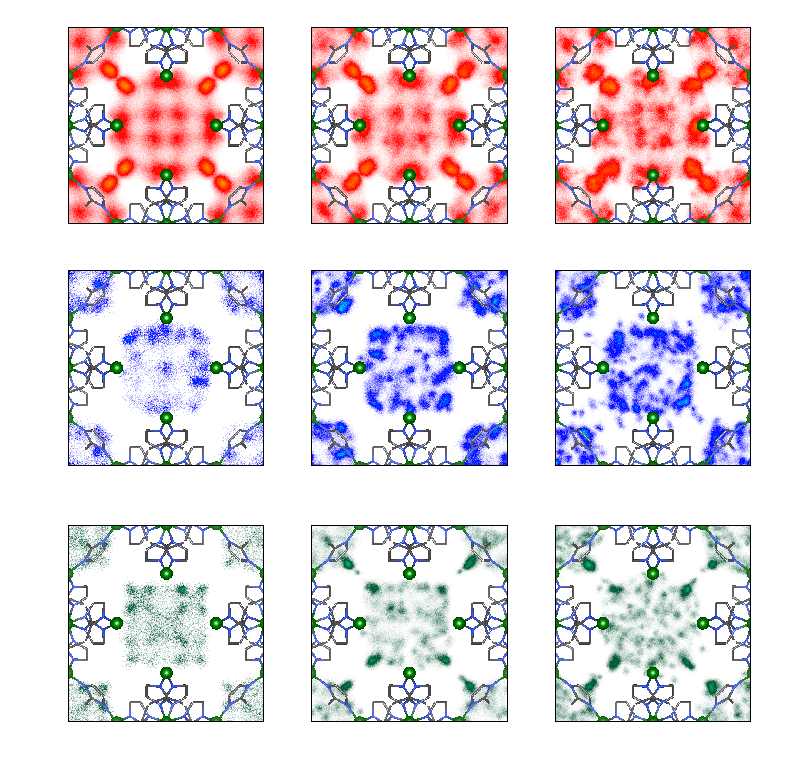
\includegraphics{licl-zif-density}}%
    \gplfronttext
  \end{picture}%
\endgroup

    \caption{Two-dimensional density profile of oxygen (top), lithium (middle) and
    chlorine (bottom) atoms in LiCl electrolyte confined in \ZIF8 at \SI{0}{GPa}
    as a function of LiCl concentration (left to right). The atoms from the
    \ZIF8 framework are superimposed, with some linkers omitted for clarity
    between the four central zinc atoms.}
    \label{fig:licl-zif:density}
\end{figure}

\begin{figure}[p]
    \centering
    % GNUPLOT: LaTeX picture with Postscript
\begingroup
  \makeatletter
  \providecommand\color[2][]{%
    \GenericError{(gnuplot) \space\space\space\@spaces}{%
      Package color not loaded in conjunction with
      terminal option `colourtext'%
    }{See the gnuplot documentation for explanation.%
    }{Either use 'blacktext' in gnuplot or load the package
      color.sty in LaTeX.}%
    \renewcommand\color[2][]{}%
  }%
  \providecommand\includegraphics[2][]{%
    \GenericError{(gnuplot) \space\space\space\@spaces}{%
      Package graphicx or graphics not loaded%
    }{See the gnuplot documentation for explanation.%
    }{The gnuplot epslatex terminal needs graphicx.sty or graphics.sty.}%
    \renewcommand\includegraphics[2][]{}%
  }%
  \providecommand\rotatebox[2]{#2}%
  \@ifundefined{ifGPcolor}{%
    \newif\ifGPcolor
    \GPcolortrue
  }{}%
  \@ifundefined{ifGPblacktext}{%
    \newif\ifGPblacktext
    \GPblacktextfalse
  }{}%
  % define a \g@addto@macro without @ in the name:
  \let\gplgaddtomacro\g@addto@macro
  % define empty templates for all commands taking text:
  \gdef\gplbacktext{}%
  \gdef\gplfronttext{}%
  \makeatother
  \ifGPblacktext
    % no textcolor at all
    \def\colorrgb#1{}%
    \def\colorgray#1{}%
  \else
    % gray or color?
    \ifGPcolor
      \def\colorrgb#1{\color[rgb]{#1}}%
      \def\colorgray#1{\color[gray]{#1}}%
      \expandafter\def\csname LTw\endcsname{\color{white}}%
      \expandafter\def\csname LTb\endcsname{\color{black}}%
      \expandafter\def\csname LTa\endcsname{\color{black}}%
      \expandafter\def\csname LT0\endcsname{\color[rgb]{1,0,0}}%
      \expandafter\def\csname LT1\endcsname{\color[rgb]{0,1,0}}%
      \expandafter\def\csname LT2\endcsname{\color[rgb]{0,0,1}}%
      \expandafter\def\csname LT3\endcsname{\color[rgb]{1,0,1}}%
      \expandafter\def\csname LT4\endcsname{\color[rgb]{0,1,1}}%
      \expandafter\def\csname LT5\endcsname{\color[rgb]{1,1,0}}%
      \expandafter\def\csname LT6\endcsname{\color[rgb]{0,0,0}}%
      \expandafter\def\csname LT7\endcsname{\color[rgb]{1,0.3,0}}%
      \expandafter\def\csname LT8\endcsname{\color[rgb]{0.5,0.5,0.5}}%
    \else
      % gray
      \def\colorrgb#1{\color{black}}%
      \def\colorgray#1{\color[gray]{#1}}%
      \expandafter\def\csname LTw\endcsname{\color{white}}%
      \expandafter\def\csname LTb\endcsname{\color{black}}%
      \expandafter\def\csname LTa\endcsname{\color{black}}%
      \expandafter\def\csname LT0\endcsname{\color{black}}%
      \expandafter\def\csname LT1\endcsname{\color{black}}%
      \expandafter\def\csname LT2\endcsname{\color{black}}%
      \expandafter\def\csname LT3\endcsname{\color{black}}%
      \expandafter\def\csname LT4\endcsname{\color{black}}%
      \expandafter\def\csname LT5\endcsname{\color{black}}%
      \expandafter\def\csname LT6\endcsname{\color{black}}%
      \expandafter\def\csname LT7\endcsname{\color{black}}%
      \expandafter\def\csname LT8\endcsname{\color{black}}%
    \fi
  \fi
    \setlength{\unitlength}{0.0500bp}%
    \ifx\gptboxheight\undefined%
      \newlength{\gptboxheight}%
      \newlength{\gptboxwidth}%
      \newsavebox{\gptboxtext}%
    \fi%
    \setlength{\fboxrule}{0.5pt}%
    \setlength{\fboxsep}{1pt}%
\begin{picture}(6500.00,12000.00)%
    \gplgaddtomacro\gplbacktext{%
    }%
    \gplgaddtomacro\gplfronttext{%
      \csname LTb\endcsname%%
      \put(1126,11693){\makebox(0,0){\strut{}\small 0 mol/L}}%
    }%
    \gplgaddtomacro\gplbacktext{%
    }%
    \gplgaddtomacro\gplfronttext{%
      \csname LTb\endcsname%%
      \put(3249,11693){\makebox(0,0){\strut{}\small 1 mol/L}}%
    }%
    \gplgaddtomacro\gplbacktext{%
    }%
    \gplgaddtomacro\gplfronttext{%
      \csname LTb\endcsname%%
      \put(5372,11693){\makebox(0,0){\strut{}\small 5 mol/L}}%
    }%
    \gplgaddtomacro\gplbacktext{%
    }%
    \gplgaddtomacro\gplfronttext{%
      \csname LTb\endcsname%%
      \put(1126,9733){\makebox(0,0){\strut{}\small 10 mol/L}}%
    }%
    \gplgaddtomacro\gplbacktext{%
    }%
    \gplgaddtomacro\gplfronttext{%
      \csname LTb\endcsname%%
      \put(3249,9733){\makebox(0,0){\strut{}\small 15 mol/L}}%
    }%
    \gplgaddtomacro\gplbacktext{%
    }%
    \gplgaddtomacro\gplfronttext{%
      \csname LTb\endcsname%%
      \put(5372,9733){\makebox(0,0){\strut{}\small 20 mol/L}}%
    }%
    \gplgaddtomacro\gplbacktext{%
    }%
    \gplgaddtomacro\gplfronttext{%
      \csname LTb\endcsname%%
      \put(3249,7773){\makebox(0,0){\strut{}\small 1 mol/L}}%
    }%
    \gplgaddtomacro\gplbacktext{%
    }%
    \gplgaddtomacro\gplfronttext{%
      \csname LTb\endcsname%%
      \put(5372,7773){\makebox(0,0){\strut{}\small 5 mol/L}}%
    }%
    \gplgaddtomacro\gplbacktext{%
    }%
    \gplgaddtomacro\gplfronttext{%
      \csname LTb\endcsname%%
      \put(1126,5813){\makebox(0,0){\strut{}\small 10 mol/L}}%
    }%
    \gplgaddtomacro\gplbacktext{%
    }%
    \gplgaddtomacro\gplfronttext{%
      \csname LTb\endcsname%%
      \put(3249,5813){\makebox(0,0){\strut{}\small 15 mol/L}}%
    }%
    \gplgaddtomacro\gplbacktext{%
    }%
    \gplgaddtomacro\gplfronttext{%
      \csname LTb\endcsname%%
      \put(5372,5813){\makebox(0,0){\strut{}\small 20 mol/L}}%
    }%
    \gplgaddtomacro\gplbacktext{%
    }%
    \gplgaddtomacro\gplfronttext{%
      \csname LTb\endcsname%%
      \put(3249,3853){\makebox(0,0){\strut{}\small 1 mol/L}}%
    }%
    \gplgaddtomacro\gplbacktext{%
    }%
    \gplgaddtomacro\gplfronttext{%
      \csname LTb\endcsname%%
      \put(5372,3853){\makebox(0,0){\strut{}\small 5 mol/L}}%
    }%
    \gplgaddtomacro\gplbacktext{%
    }%
    \gplgaddtomacro\gplfronttext{%
      \csname LTb\endcsname%%
      \put(1126,1893){\makebox(0,0){\strut{}\small 10 mol/L}}%
    }%
    \gplgaddtomacro\gplbacktext{%
    }%
    \gplgaddtomacro\gplfronttext{%
      \csname LTb\endcsname%%
      \put(3249,1893){\makebox(0,0){\strut{}\small 15 mol/L}}%
    }%
    \gplgaddtomacro\gplbacktext{%
    }%
    \gplgaddtomacro\gplfronttext{%
      \csname LTb\endcsname%%
      \put(5372,1893){\makebox(0,0){\strut{}\small 20 mol/L}}%
    }%
    \gplbacktext
    \put(0,0){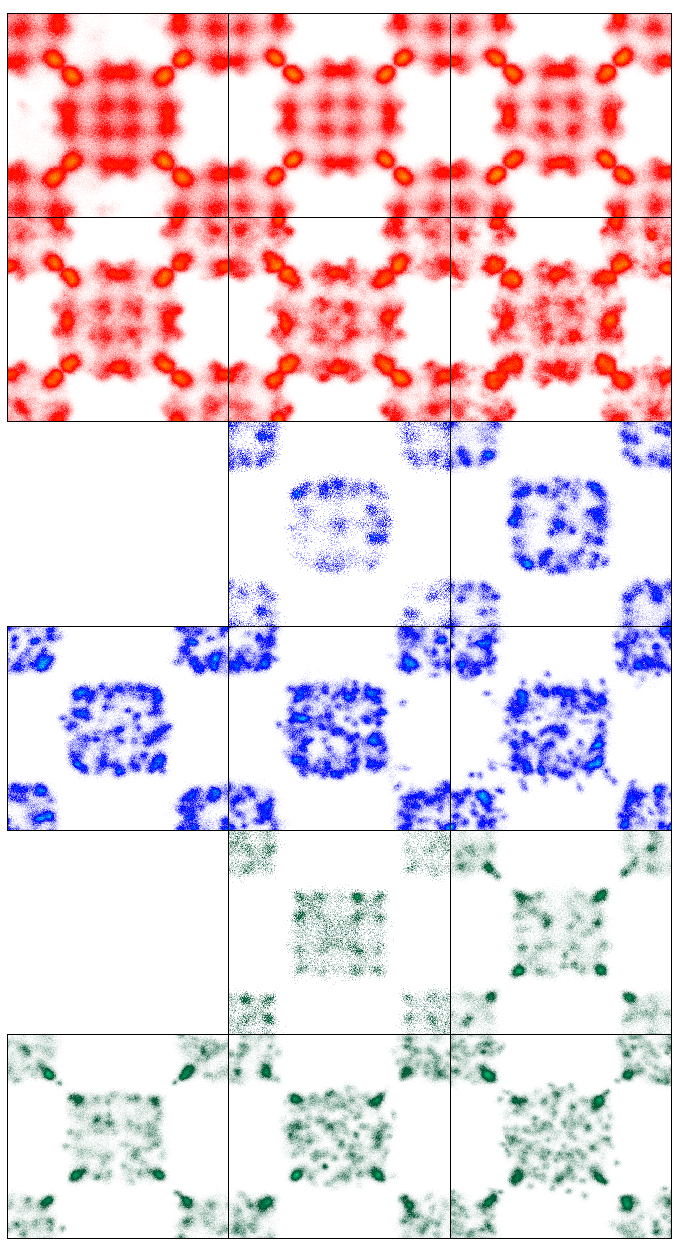
\includegraphics{licl-zif-density-all}}%
    \gplfronttext
  \end{picture}%
\endgroup

    \caption{2 dimensional density profile of oxygen (red), lithium (blue) and
    chlorine (green) atoms in LiCl electrolyte confined in \ZIF8 at \SI{0}{GPa}
    as a function of LiCl concentration. Every graph is presented in fractional
    coordinates between -0.5 and 0.5.}
    \label{fig:licl-zif:density:all}
\end{figure}


We also present in figure~\ref{fig:licl-zif:density} the density profile of atoms in the
confined liquid, represented in the $xy$ plane, averaged over $z$ and the
$3\times3\times3$ super-cell. To account for cell deformation during the $(N, P, T)$
simulations, we used fractional coordinates to represent the positions of atoms.

Here we clearly see the long distance structuration of water inside the \ZIF8
pores. At low concentration (\SI{1}{mol/L}), the water molecules occupy very
well-defined sites, in particular inside the windows between two neighboring
cages. As the concentration increases, this organization is perturbed by the
ions inserted in the water molecules' network --- however this effect is
relatively small, and the water distribution is not greatly affected. The same
can be observed in the distribution of chlorine ions, with a well defined, high
symmetry distribution at low concentration, but as the concentration increases
the distribution of ions becomes more and more distributed over the whole pore
space. Concerning lithium ions, they present a looser arrangement inside the
pores, and are distributed relatively evenly, yet present a preferential
occupation next to the water molecules in the 6-member windows (in the diagonal
in figure~\ref{fig:licl-zif:density}).

These results can be explained by both the difference in kinetic
radius\cite{Marcus1988} for water molecules (\SI{2.65}{\angstrom}), chlorine
ions (\SI{3.2}{\angstrom}) and lithium ions (\SI{2.1}{\angstrom}), as well as
the strong attraction between water oxygen atoms and lithium. The difference in
size allows lithium ions to fit in smaller spaces, and an even distribution of
ions will increase the total entropy of the system. At the same time, chlorine
ions and water molecules are more polarizable than lithium, and as such will
have stronger interactions with the aromatic linkers, making it preferable for
them to take the highly organized arrangement we observe.

\subsection{Dynamics under confinement}

In order to characterize the dynamic of water confined in \ZIF8 and the impact
of LiCl concentration and pressure on this dynamic, we used two different
indicators to quantify the adsorbed molecules' dynamics. The first one is based
on the lifetime of hydrogen bonds between water molecules, detected by a
geometric criterion: following \citeauthor{Luzar1996}\cite{Luzar1996}, we
characterize the presence of a hydrogen bond between two water molecules as two
oxygen atoms separated by less than \SI{3.5}{\angstrom}, with an
oxygen--oxygen--hydrogen ($\widehat{\text{OOH}}$) angle less than 30\textdegree.
We then computed the time autocorrelation function of the hydrogen bond
existence functions $H(t)$ --- set to 1 if the bond exists at time $t$, 0 if is
does not exists --- as:
\[C_{\text{hbonds}}(t) = \left\langle H(t_0) \cdot H(t_0 + t) \right\rangle_{t_0} \]
The decay of this autocorrelation function, presented in
figure~\ref{fig:licl-zif:hbonds}, is characteristic of the dynamics of the hydrogen bond
network and the lifetime of individual H bonds.

This geometric definition of hydrogen bonds has a minor inconvenient: small
fluctuations of the atomic positions, near the cut-off values, can be mistaken
for H bond formation and breaking. To overcome this issue, we also computed the
time autocorrelation of the orientation vector, $\vec u(t)$, of water molecules:
\[C_{\text{rot}}(t) = \left\langle P_2(\vec u(t_0) \cdot \vec u(t_0 + t)) \right\rangle_{t_0} ,\]
where $P_2(x)$ is the second order Legendre polynomial $P_2(x) = \frac{1}{2}
(3x^2 - 1)$\cite{Fogarty2014}. The results for rotational correlation are
presented in supporting information figure~\ref{fig:licl-zif:rotcf} and
table~\ref{table:licl-zif:rotcf}. Because water is a strongly associated liquid,
breaking a hydrogen bond is predominantly correlated to rotational jumps, both
autocorrelation curves behave in very similar ways, and we focus here the discussion
on hydrogen bonds decays.

\begin{figure}[ht]
    \centering
    % GNUPLOT: LaTeX picture with Postscript
\begingroup
  \makeatletter
  \providecommand\color[2][]{%
    \GenericError{(gnuplot) \space\space\space\@spaces}{%
      Package color not loaded in conjunction with
      terminal option `colourtext'%
    }{See the gnuplot documentation for explanation.%
    }{Either use 'blacktext' in gnuplot or load the package
      color.sty in LaTeX.}%
    \renewcommand\color[2][]{}%
  }%
  \providecommand\includegraphics[2][]{%
    \GenericError{(gnuplot) \space\space\space\@spaces}{%
      Package graphicx or graphics not loaded%
    }{See the gnuplot documentation for explanation.%
    }{The gnuplot epslatex terminal needs graphicx.sty or graphics.sty.}%
    \renewcommand\includegraphics[2][]{}%
  }%
  \providecommand\rotatebox[2]{#2}%
  \@ifundefined{ifGPcolor}{%
    \newif\ifGPcolor
    \GPcolortrue
  }{}%
  \@ifundefined{ifGPblacktext}{%
    \newif\ifGPblacktext
    \GPblacktextfalse
  }{}%
  % define a \g@addto@macro without @ in the name:
  \let\gplgaddtomacro\g@addto@macro
  % define empty templates for all commands taking text:
  \gdef\gplbacktext{}%
  \gdef\gplfronttext{}%
  \makeatother
  \ifGPblacktext
    % no textcolor at all
    \def\colorrgb#1{}%
    \def\colorgray#1{}%
  \else
    % gray or color?
    \ifGPcolor
      \def\colorrgb#1{\color[rgb]{#1}}%
      \def\colorgray#1{\color[gray]{#1}}%
      \expandafter\def\csname LTw\endcsname{\color{white}}%
      \expandafter\def\csname LTb\endcsname{\color{black}}%
      \expandafter\def\csname LTa\endcsname{\color{black}}%
      \expandafter\def\csname LT0\endcsname{\color[rgb]{1,0,0}}%
      \expandafter\def\csname LT1\endcsname{\color[rgb]{0,1,0}}%
      \expandafter\def\csname LT2\endcsname{\color[rgb]{0,0,1}}%
      \expandafter\def\csname LT3\endcsname{\color[rgb]{1,0,1}}%
      \expandafter\def\csname LT4\endcsname{\color[rgb]{0,1,1}}%
      \expandafter\def\csname LT5\endcsname{\color[rgb]{1,1,0}}%
      \expandafter\def\csname LT6\endcsname{\color[rgb]{0,0,0}}%
      \expandafter\def\csname LT7\endcsname{\color[rgb]{1,0.3,0}}%
      \expandafter\def\csname LT8\endcsname{\color[rgb]{0.5,0.5,0.5}}%
    \else
      % gray
      \def\colorrgb#1{\color{black}}%
      \def\colorgray#1{\color[gray]{#1}}%
      \expandafter\def\csname LTw\endcsname{\color{white}}%
      \expandafter\def\csname LTb\endcsname{\color{black}}%
      \expandafter\def\csname LTa\endcsname{\color{black}}%
      \expandafter\def\csname LT0\endcsname{\color{black}}%
      \expandafter\def\csname LT1\endcsname{\color{black}}%
      \expandafter\def\csname LT2\endcsname{\color{black}}%
      \expandafter\def\csname LT3\endcsname{\color{black}}%
      \expandafter\def\csname LT4\endcsname{\color{black}}%
      \expandafter\def\csname LT5\endcsname{\color{black}}%
      \expandafter\def\csname LT6\endcsname{\color{black}}%
      \expandafter\def\csname LT7\endcsname{\color{black}}%
      \expandafter\def\csname LT8\endcsname{\color{black}}%
    \fi
  \fi
    \setlength{\unitlength}{0.0500bp}%
    \ifx\gptboxheight\undefined%
      \newlength{\gptboxheight}%
      \newlength{\gptboxwidth}%
      \newsavebox{\gptboxtext}%
    \fi%
    \setlength{\fboxrule}{0.5pt}%
    \setlength{\fboxsep}{1pt}%
\begin{picture}(5660.00,5660.00)%
    \gplgaddtomacro\gplbacktext{%
      \csname LTb\endcsname%%
      \put(752,3264){\makebox(0,0)[r]{\strut{}$0$}}%
      \csname LTb\endcsname%%
      \put(752,3700){\makebox(0,0)[r]{\strut{}$0.2$}}%
      \csname LTb\endcsname%%
      \put(752,4135){\makebox(0,0)[r]{\strut{}$0.4$}}%
      \csname LTb\endcsname%%
      \put(752,4571){\makebox(0,0)[r]{\strut{}$0.6$}}%
      \csname LTb\endcsname%%
      \put(752,5006){\makebox(0,0)[r]{\strut{}$0.8$}}%
      \csname LTb\endcsname%%
      \put(752,5442){\makebox(0,0)[r]{\strut{}$1$}}%
      \csname LTb\endcsname%%
      \put(871,3047){\makebox(0,0){\strut{}$0$}}%
      \csname LTb\endcsname%%
      \put(1979,3047){\makebox(0,0){\strut{}$5$}}%
      \csname LTb\endcsname%%
      \put(3087,3047){\makebox(0,0){\strut{}$10$}}%
      \csname LTb\endcsname%%
      \put(4194,3047){\makebox(0,0){\strut{}$15$}}%
      \csname LTb\endcsname%%
      \put(5302,3047){\makebox(0,0){\strut{}$20$}}%
    }%
    \gplgaddtomacro\gplfronttext{%
      \csname LTb\endcsname%%
      \put(178,4353){\rotatebox{-270}{\makebox(0,0){\strut{}auto correlation}}}%
      \csname LTb\endcsname%%
      \put(2631,5247){\makebox(0,0)[r]{\strut{}0 mol/L}}%
      \csname LTb\endcsname%%
      \put(2631,5030){\makebox(0,0)[r]{\strut{}1 mol/L}}%
      \csname LTb\endcsname%%
      \put(2631,4813){\makebox(0,0)[r]{\strut{}5 mol/L}}%
      \csname LTb\endcsname%%
      \put(4383,5247){\makebox(0,0)[r]{\strut{}10 mol/L}}%
      \csname LTb\endcsname%%
      \put(4383,5030){\makebox(0,0)[r]{\strut{}15 mol/L}}%
      \csname LTb\endcsname%%
      \put(4383,4813){\makebox(0,0)[r]{\strut{}20 mol/L}}%
    }%
    \gplgaddtomacro\gplbacktext{%
      \csname LTb\endcsname%%
      \put(752,694){\makebox(0,0)[r]{\strut{}$0$}}%
      \csname LTb\endcsname%%
      \put(752,1078){\makebox(0,0)[r]{\strut{}$0.2$}}%
      \csname LTb\endcsname%%
      \put(752,1462){\makebox(0,0)[r]{\strut{}$0.4$}}%
      \csname LTb\endcsname%%
      \put(752,1845){\makebox(0,0)[r]{\strut{}$0.6$}}%
      \csname LTb\endcsname%%
      \put(752,2229){\makebox(0,0)[r]{\strut{}$0.8$}}%
      \csname LTb\endcsname%%
      \put(752,2613){\makebox(0,0)[r]{\strut{}$1$}}%
      \csname LTb\endcsname%%
      \put(871,477){\makebox(0,0){\strut{}$0$}}%
      \csname LTb\endcsname%%
      \put(1979,477){\makebox(0,0){\strut{}$5$}}%
      \csname LTb\endcsname%%
      \put(3087,477){\makebox(0,0){\strut{}$10$}}%
      \csname LTb\endcsname%%
      \put(4194,477){\makebox(0,0){\strut{}$15$}}%
      \csname LTb\endcsname%%
      \put(5302,477){\makebox(0,0){\strut{}$20$}}%
    }%
    \gplgaddtomacro\gplfronttext{%
      \csname LTb\endcsname%%
      \put(178,1653){\rotatebox{-270}{\makebox(0,0){\strut{}auto correlation}}}%
      \csname LTb\endcsname%%
      \put(3086,152){\makebox(0,0){\strut{}time (ps)}}%
    }%
    \gplbacktext
    \put(0,0){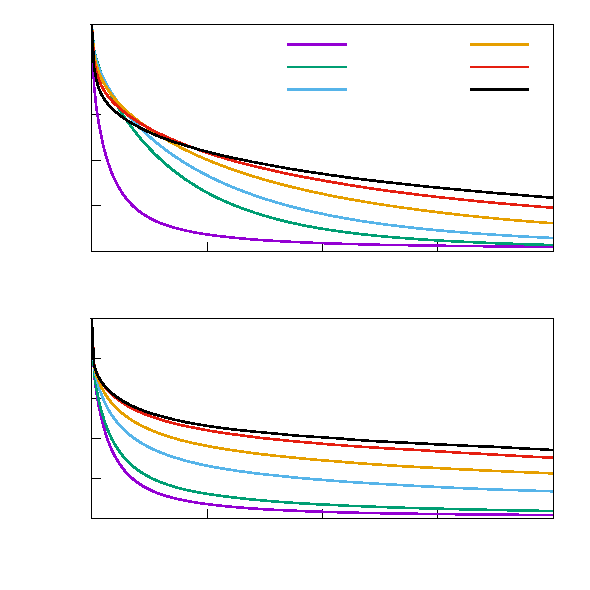
\includegraphics{licl-zif-hbonds}}%
    \gplfronttext
  \end{picture}%
\endgroup

    \caption{Hydrogen bonds existence autocorrelation in bulk (top) and
    confined (bottom) electrolyte as function of LiCl concentration.}
    \label{fig:licl-zif:hbonds}
\end{figure}

We then fitted all the autocorrelation functions with bi-exponential functions:
\[ f(t) = A_1 e^{-t / \tau_1} + A_2 e^{-t / \tau_2}, \]
where $\tau_1$ and $\tau_2$ are the two time scales of decay, and $A_1$ and
$A_2$ are their relative weights. The resulting fit parameters are presented in
supporting information table~\ref{table:licl-zif:hbonds}, together with the fit
procedure and error estimates. The corresponding data is presented in
figure~\ref{fig:licl-zif:hbonds:fit} at the pressure of \SI{0}{GPa}. We found that the
pressure only have a negligible influence on both the lifetimes and the weights
of these lifetimes. Similar curves for all pressures are presented in
supplementary information figure~\ref{fig:licl-zif:hbonds:fit:pressure}.

\begin{figure}[ht]
    \centering
    % GNUPLOT: LaTeX picture with Postscript
\begingroup
  \makeatletter
  \providecommand\color[2][]{%
    \GenericError{(gnuplot) \space\space\space\@spaces}{%
      Package color not loaded in conjunction with
      terminal option `colourtext'%
    }{See the gnuplot documentation for explanation.%
    }{Either use 'blacktext' in gnuplot or load the package
      color.sty in LaTeX.}%
    \renewcommand\color[2][]{}%
  }%
  \providecommand\includegraphics[2][]{%
    \GenericError{(gnuplot) \space\space\space\@spaces}{%
      Package graphicx or graphics not loaded%
    }{See the gnuplot documentation for explanation.%
    }{The gnuplot epslatex terminal needs graphicx.sty or graphics.sty.}%
    \renewcommand\includegraphics[2][]{}%
  }%
  \providecommand\rotatebox[2]{#2}%
  \@ifundefined{ifGPcolor}{%
    \newif\ifGPcolor
    \GPcolortrue
  }{}%
  \@ifundefined{ifGPblacktext}{%
    \newif\ifGPblacktext
    \GPblacktextfalse
  }{}%
  % define a \g@addto@macro without @ in the name:
  \let\gplgaddtomacro\g@addto@macro
  % define empty templates for all commands taking text:
  \gdef\gplbacktext{}%
  \gdef\gplfronttext{}%
  \makeatother
  \ifGPblacktext
    % no textcolor at all
    \def\colorrgb#1{}%
    \def\colorgray#1{}%
  \else
    % gray or color?
    \ifGPcolor
      \def\colorrgb#1{\color[rgb]{#1}}%
      \def\colorgray#1{\color[gray]{#1}}%
      \expandafter\def\csname LTw\endcsname{\color{white}}%
      \expandafter\def\csname LTb\endcsname{\color{black}}%
      \expandafter\def\csname LTa\endcsname{\color{black}}%
      \expandafter\def\csname LT0\endcsname{\color[rgb]{1,0,0}}%
      \expandafter\def\csname LT1\endcsname{\color[rgb]{0,1,0}}%
      \expandafter\def\csname LT2\endcsname{\color[rgb]{0,0,1}}%
      \expandafter\def\csname LT3\endcsname{\color[rgb]{1,0,1}}%
      \expandafter\def\csname LT4\endcsname{\color[rgb]{0,1,1}}%
      \expandafter\def\csname LT5\endcsname{\color[rgb]{1,1,0}}%
      \expandafter\def\csname LT6\endcsname{\color[rgb]{0,0,0}}%
      \expandafter\def\csname LT7\endcsname{\color[rgb]{1,0.3,0}}%
      \expandafter\def\csname LT8\endcsname{\color[rgb]{0.5,0.5,0.5}}%
    \else
      % gray
      \def\colorrgb#1{\color{black}}%
      \def\colorgray#1{\color[gray]{#1}}%
      \expandafter\def\csname LTw\endcsname{\color{white}}%
      \expandafter\def\csname LTb\endcsname{\color{black}}%
      \expandafter\def\csname LTa\endcsname{\color{black}}%
      \expandafter\def\csname LT0\endcsname{\color{black}}%
      \expandafter\def\csname LT1\endcsname{\color{black}}%
      \expandafter\def\csname LT2\endcsname{\color{black}}%
      \expandafter\def\csname LT3\endcsname{\color{black}}%
      \expandafter\def\csname LT4\endcsname{\color{black}}%
      \expandafter\def\csname LT5\endcsname{\color{black}}%
      \expandafter\def\csname LT6\endcsname{\color{black}}%
      \expandafter\def\csname LT7\endcsname{\color{black}}%
      \expandafter\def\csname LT8\endcsname{\color{black}}%
    \fi
  \fi
    \setlength{\unitlength}{0.0500bp}%
    \ifx\gptboxheight\undefined%
      \newlength{\gptboxheight}%
      \newlength{\gptboxwidth}%
      \newsavebox{\gptboxtext}%
    \fi%
    \setlength{\fboxrule}{0.5pt}%
    \setlength{\fboxsep}{1pt}%
\begin{picture}(7580.00,3960.00)%
    \gplgaddtomacro\gplbacktext{%
      \csname LTb\endcsname%%
      \put(612,2352){\makebox(0,0)[r]{\strut{}$0$}}%
      \csname LTb\endcsname%%
      \put(612,2707){\makebox(0,0)[r]{\strut{}$1$}}%
      \csname LTb\endcsname%%
      \put(612,3063){\makebox(0,0)[r]{\strut{}$2$}}%
      \csname LTb\endcsname%%
      \put(612,3418){\makebox(0,0)[r]{\strut{}$3$}}%
      \csname LTb\endcsname%%
      \put(612,3773){\makebox(0,0)[r]{\strut{}$4$}}%
      \csname LTb\endcsname%%
      \put(714,2166){\makebox(0,0){\strut{}$0$}}%
      \csname LTb\endcsname%%
      \put(1406,2166){\makebox(0,0){\strut{}$5$}}%
      \csname LTb\endcsname%%
      \put(2099,2166){\makebox(0,0){\strut{}$10$}}%
      \csname LTb\endcsname%%
      \put(2791,2166){\makebox(0,0){\strut{}$15$}}%
      \csname LTb\endcsname%%
      \put(3483,2166){\makebox(0,0){\strut{}$20$}}%
    }%
    \gplgaddtomacro\gplfronttext{%
      \csname LTb\endcsname%%
      \put(222,3062){\rotatebox{-270}{\makebox(0,0){\strut{}$\tau_1$ (ps)}}}%
    }%
    \gplgaddtomacro\gplbacktext{%
      \csname LTb\endcsname%%
      \put(4402,2352){\makebox(0,0)[r]{\strut{}$0$}}%
      \csname LTb\endcsname%%
      \put(4402,2707){\makebox(0,0)[r]{\strut{}$20$}}%
      \csname LTb\endcsname%%
      \put(4402,3063){\makebox(0,0)[r]{\strut{}$40$}}%
      \csname LTb\endcsname%%
      \put(4402,3418){\makebox(0,0)[r]{\strut{}$60$}}%
      \csname LTb\endcsname%%
      \put(4402,3773){\makebox(0,0)[r]{\strut{}$80$}}%
      \csname LTb\endcsname%%
      \put(4504,2166){\makebox(0,0){\strut{}$0$}}%
      \csname LTb\endcsname%%
      \put(5196,2166){\makebox(0,0){\strut{}$5$}}%
      \csname LTb\endcsname%%
      \put(5889,2166){\makebox(0,0){\strut{}$10$}}%
      \csname LTb\endcsname%%
      \put(6581,2166){\makebox(0,0){\strut{}$15$}}%
      \csname LTb\endcsname%%
      \put(7273,2166){\makebox(0,0){\strut{}$20$}}%
    }%
    \gplgaddtomacro\gplfronttext{%
      \csname LTb\endcsname%%
      \put(3910,3062){\rotatebox{-270}{\makebox(0,0){\strut{}$\tau_2$ (ps)}}}%
      \csname LTb\endcsname%%
      \put(5422,3606){\makebox(0,0)[r]{\strut{}confined}}%
      \csname LTb\endcsname%%
      \put(5422,3420){\makebox(0,0)[r]{\strut{}bulk}}%
    }%
    \gplgaddtomacro\gplbacktext{%
      \csname LTb\endcsname%%
      \put(612,595){\makebox(0,0)[r]{\strut{}$0$}}%
      \csname LTb\endcsname%%
      \put(612,895){\makebox(0,0)[r]{\strut{}$25$}}%
      \csname LTb\endcsname%%
      \put(612,1195){\makebox(0,0)[r]{\strut{}$50$}}%
      \csname LTb\endcsname%%
      \put(612,1494){\makebox(0,0)[r]{\strut{}$75$}}%
      \csname LTb\endcsname%%
      \put(612,1794){\makebox(0,0)[r]{\strut{}$100$}}%
      \csname LTb\endcsname%%
      \put(714,409){\makebox(0,0){\strut{}$0$}}%
      \csname LTb\endcsname%%
      \put(1406,409){\makebox(0,0){\strut{}$5$}}%
      \csname LTb\endcsname%%
      \put(2099,409){\makebox(0,0){\strut{}$10$}}%
      \csname LTb\endcsname%%
      \put(2791,409){\makebox(0,0){\strut{}$15$}}%
      \csname LTb\endcsname%%
      \put(3483,409){\makebox(0,0){\strut{}$20$}}%
    }%
    \gplgaddtomacro\gplfronttext{%
      \csname LTb\endcsname%%
      \put(201,1194){\rotatebox{-270}{\makebox(0,0){\strut{}$A_1$ (\%)}}}%
      \csname LTb\endcsname%%
      \put(2098,130){\makebox(0,0){\strut{}\small concentration (mol/L)}}%
    }%
    \gplgaddtomacro\gplbacktext{%
      \csname LTb\endcsname%%
      \put(4402,595){\makebox(0,0)[r]{\strut{}$0$}}%
      \csname LTb\endcsname%%
      \put(4402,895){\makebox(0,0)[r]{\strut{}$25$}}%
      \csname LTb\endcsname%%
      \put(4402,1195){\makebox(0,0)[r]{\strut{}$50$}}%
      \csname LTb\endcsname%%
      \put(4402,1494){\makebox(0,0)[r]{\strut{}$75$}}%
      \csname LTb\endcsname%%
      \put(4402,1794){\makebox(0,0)[r]{\strut{}$100$}}%
      \csname LTb\endcsname%%
      \put(4504,409){\makebox(0,0){\strut{}$0$}}%
      \csname LTb\endcsname%%
      \put(5196,409){\makebox(0,0){\strut{}$5$}}%
      \csname LTb\endcsname%%
      \put(5889,409){\makebox(0,0){\strut{}$10$}}%
      \csname LTb\endcsname%%
      \put(6581,409){\makebox(0,0){\strut{}$15$}}%
      \csname LTb\endcsname%%
      \put(7273,409){\makebox(0,0){\strut{}$20$}}%
    }%
    \gplgaddtomacro\gplfronttext{%
      \csname LTb\endcsname%%
      \put(3991,1194){\rotatebox{-270}{\makebox(0,0){\strut{}$A_2$ (\%)}}}%
      \csname LTb\endcsname%%
      \put(5888,130){\makebox(0,0){\strut{}\small concentration (mol/L)}}%
    }%
    \gplbacktext
    \put(0,0){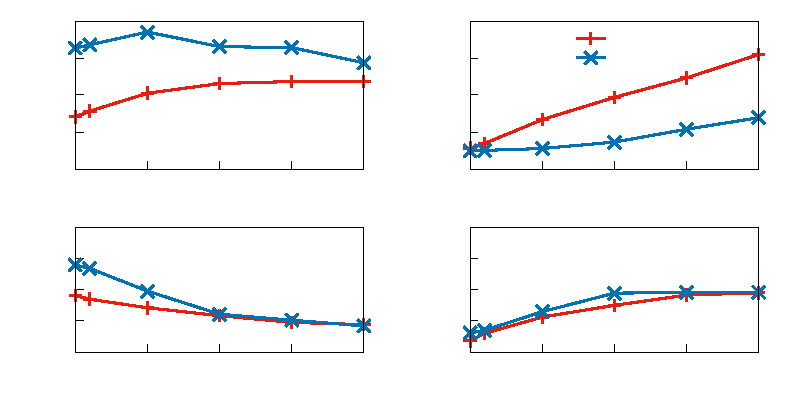
\includegraphics{licl-zif-hbonds-fit}}%
    \gplfronttext
  \end{picture}%
\endgroup

    \caption{Variations of the time constant and weights of the bi-exponential
    hydrogen bonds autocorrelation decay at \SI{0}{GPa} in bulk and confined
    liquid as function of the LiCl concentration.}
    \label{fig:licl-zif:hbonds:fit}
\end{figure}

\begin{table}[ht]
    \caption{Fit coefficients for the hydrogen bonds autocorrelation decay.}
    \label{table:licl-zif:hbonds}
    \centering
    \renewcommand{\arraystretch}{1.3}
    \begin{tabular}{c c c c c c c c c c}
        \toprule
        \multicolumn{1}{c}{~} & \multicolumn{4}{c}{Bulk}                          &~& \multicolumn{4}{c}{Confined} \\
        \multicolumn{1}{c}{~} & $\tau_1$ (ps) & $\tau_2$ (ps) & $A_1$   & $A_2$   &~& $\tau_1$ (ps) & $\tau_2$ (ps) & $A_1$   & $A_2$   \\
        \midrule
        \SI{0}{mol/L}         &    3.27       &    9.84       & 69.7 \% & 15.4 \% &~&  1.41         &  11.3         & 45.2 \% & 8.94 \% \\
        \SI{1}{mol/L}         &    3.36       &    10.1       & 67.0 \% & 17.3 \% &~&  1.56         &  13.8         & 42.3 \% & 15.0 \% \\
        \SI{5}{mol/L}         &    3.70       &    11.1       & 48.8 \% & 32.4 \% &~&  2.05         &  26.8         & 35.4 \% & 28.0 \% \\
        \SI{10}{mol/L}        &    3.31       &    14.6       & 30.3 \% & 47.2 \% &~&  2.31         &  38.7         & 29.1 \% & 37.4 \% \\
        \SI{15}{mol/L}        &    3.28       &    21.5       & 25.5 \% & 47.6 \% &~&  2.37         &  49.3         & 23.8 \% & 45.7 \% \\
        \SI{20}{mol/L}        &    2.87       &    27.7       & 20.9 \% & 47.9 \% &~&  2.36         &  61.9         & 22.0 \% & 47.5 \% \\
        \bottomrule
    \end{tabular}
\end{table}

\begin{figure}[ht]
    \centering
    % GNUPLOT: LaTeX picture with Postscript
\begingroup
  \makeatletter
  \providecommand\color[2][]{%
    \GenericError{(gnuplot) \space\space\space\@spaces}{%
      Package color not loaded in conjunction with
      terminal option `colourtext'%
    }{See the gnuplot documentation for explanation.%
    }{Either use 'blacktext' in gnuplot or load the package
      color.sty in LaTeX.}%
    \renewcommand\color[2][]{}%
  }%
  \providecommand\includegraphics[2][]{%
    \GenericError{(gnuplot) \space\space\space\@spaces}{%
      Package graphicx or graphics not loaded%
    }{See the gnuplot documentation for explanation.%
    }{The gnuplot epslatex terminal needs graphicx.sty or graphics.sty.}%
    \renewcommand\includegraphics[2][]{}%
  }%
  \providecommand\rotatebox[2]{#2}%
  \@ifundefined{ifGPcolor}{%
    \newif\ifGPcolor
    \GPcolortrue
  }{}%
  \@ifundefined{ifGPblacktext}{%
    \newif\ifGPblacktext
    \GPblacktextfalse
  }{}%
  % define a \g@addto@macro without @ in the name:
  \let\gplgaddtomacro\g@addto@macro
  % define empty templates for all commands taking text:
  \gdef\gplbacktext{}%
  \gdef\gplfronttext{}%
  \makeatother
  \ifGPblacktext
    % no textcolor at all
    \def\colorrgb#1{}%
    \def\colorgray#1{}%
  \else
    % gray or color?
    \ifGPcolor
      \def\colorrgb#1{\color[rgb]{#1}}%
      \def\colorgray#1{\color[gray]{#1}}%
      \expandafter\def\csname LTw\endcsname{\color{white}}%
      \expandafter\def\csname LTb\endcsname{\color{black}}%
      \expandafter\def\csname LTa\endcsname{\color{black}}%
      \expandafter\def\csname LT0\endcsname{\color[rgb]{1,0,0}}%
      \expandafter\def\csname LT1\endcsname{\color[rgb]{0,1,0}}%
      \expandafter\def\csname LT2\endcsname{\color[rgb]{0,0,1}}%
      \expandafter\def\csname LT3\endcsname{\color[rgb]{1,0,1}}%
      \expandafter\def\csname LT4\endcsname{\color[rgb]{0,1,1}}%
      \expandafter\def\csname LT5\endcsname{\color[rgb]{1,1,0}}%
      \expandafter\def\csname LT6\endcsname{\color[rgb]{0,0,0}}%
      \expandafter\def\csname LT7\endcsname{\color[rgb]{1,0.3,0}}%
      \expandafter\def\csname LT8\endcsname{\color[rgb]{0.5,0.5,0.5}}%
    \else
      % gray
      \def\colorrgb#1{\color{black}}%
      \def\colorgray#1{\color[gray]{#1}}%
      \expandafter\def\csname LTw\endcsname{\color{white}}%
      \expandafter\def\csname LTb\endcsname{\color{black}}%
      \expandafter\def\csname LTa\endcsname{\color{black}}%
      \expandafter\def\csname LT0\endcsname{\color{black}}%
      \expandafter\def\csname LT1\endcsname{\color{black}}%
      \expandafter\def\csname LT2\endcsname{\color{black}}%
      \expandafter\def\csname LT3\endcsname{\color{black}}%
      \expandafter\def\csname LT4\endcsname{\color{black}}%
      \expandafter\def\csname LT5\endcsname{\color{black}}%
      \expandafter\def\csname LT6\endcsname{\color{black}}%
      \expandafter\def\csname LT7\endcsname{\color{black}}%
      \expandafter\def\csname LT8\endcsname{\color{black}}%
    \fi
  \fi
    \setlength{\unitlength}{0.0500bp}%
    \ifx\gptboxheight\undefined%
      \newlength{\gptboxheight}%
      \newlength{\gptboxwidth}%
      \newsavebox{\gptboxtext}%
    \fi%
    \setlength{\fboxrule}{0.5pt}%
    \setlength{\fboxsep}{1pt}%
\begin{picture}(7580.00,5100.00)%
    \gplgaddtomacro\gplbacktext{%
      \csname LTb\endcsname%%
      \put(408,2667){\makebox(0,0)[r]{\strut{}$0$}}%
      \csname LTb\endcsname%%
      \put(408,3037){\makebox(0,0)[r]{\strut{}$1$}}%
      \csname LTb\endcsname%%
      \put(408,3408){\makebox(0,0)[r]{\strut{}$2$}}%
      \csname LTb\endcsname%%
      \put(408,3778){\makebox(0,0)[r]{\strut{}$3$}}%
      \csname LTb\endcsname%%
      \put(408,4148){\makebox(0,0)[r]{\strut{}$4$}}%
      \csname LTb\endcsname%%
      \put(510,2481){\makebox(0,0){\strut{}$0$}}%
      \csname LTb\endcsname%%
      \put(1253,2481){\makebox(0,0){\strut{}$5$}}%
      \csname LTb\endcsname%%
      \put(1997,2481){\makebox(0,0){\strut{}$10$}}%
      \csname LTb\endcsname%%
      \put(2740,2481){\makebox(0,0){\strut{}$15$}}%
      \csname LTb\endcsname%%
      \put(3483,2481){\makebox(0,0){\strut{}$20$}}%
    }%
    \gplgaddtomacro\gplfronttext{%
      \csname LTb\endcsname%%
      \put(120,3407){\rotatebox{-270}{\makebox(0,0){\strut{}$\tau_1$ (ps)}}}%
      \csname LTb\endcsname%%
      \put(1137,4440){\makebox(0,0){\strut{}\footnotesize 0}}%
      \csname LTb\endcsname%%
      \put(1768,4440){\makebox(0,0){\strut{}\footnotesize 0.33}}%
      \csname LTb\endcsname%%
      \put(2399,4440){\makebox(0,0){\strut{}\footnotesize 0.67}}%
      \csname LTb\endcsname%%
      \put(3031,4440){\makebox(0,0){\strut{}\footnotesize 1}}%
      \csname LTb\endcsname%%
      \put(2084,5016){\makebox(0,0){\strut{}\footnotesize bulk liquid pressure (GPa)}}%
    }%
    \gplgaddtomacro\gplbacktext{%
      \csname LTb\endcsname%%
      \put(4198,2667){\makebox(0,0)[r]{\strut{}$0$}}%
      \csname LTb\endcsname%%
      \put(4198,3037){\makebox(0,0)[r]{\strut{}$25$}}%
      \csname LTb\endcsname%%
      \put(4198,3408){\makebox(0,0)[r]{\strut{}$50$}}%
      \csname LTb\endcsname%%
      \put(4198,3778){\makebox(0,0)[r]{\strut{}$75$}}%
      \csname LTb\endcsname%%
      \put(4198,4148){\makebox(0,0)[r]{\strut{}$100$}}%
      \csname LTb\endcsname%%
      \put(4300,2481){\makebox(0,0){\strut{}$0$}}%
      \csname LTb\endcsname%%
      \put(5043,2481){\makebox(0,0){\strut{}$5$}}%
      \csname LTb\endcsname%%
      \put(5787,2481){\makebox(0,0){\strut{}$10$}}%
      \csname LTb\endcsname%%
      \put(6530,2481){\makebox(0,0){\strut{}$15$}}%
      \csname LTb\endcsname%%
      \put(7273,2481){\makebox(0,0){\strut{}$20$}}%
    }%
    \gplgaddtomacro\gplfronttext{%
      \csname LTb\endcsname%%
      \put(3808,3407){\rotatebox{-270}{\makebox(0,0){\strut{}$\tau_2$ (ps)}}}%
    }%
    \gplgaddtomacro\gplbacktext{%
      \csname LTb\endcsname%%
      \put(408,627){\makebox(0,0)[r]{\strut{}$0$}}%
      \csname LTb\endcsname%%
      \put(408,998){\makebox(0,0)[r]{\strut{}$25$}}%
      \csname LTb\endcsname%%
      \put(408,1368){\makebox(0,0)[r]{\strut{}$50$}}%
      \csname LTb\endcsname%%
      \put(408,1739){\makebox(0,0)[r]{\strut{}$75$}}%
      \csname LTb\endcsname%%
      \put(408,2109){\makebox(0,0)[r]{\strut{}$100$}}%
      \csname LTb\endcsname%%
      \put(510,441){\makebox(0,0){\strut{}$0$}}%
      \csname LTb\endcsname%%
      \put(1253,441){\makebox(0,0){\strut{}$5$}}%
      \csname LTb\endcsname%%
      \put(1997,441){\makebox(0,0){\strut{}$10$}}%
      \csname LTb\endcsname%%
      \put(2740,441){\makebox(0,0){\strut{}$15$}}%
      \csname LTb\endcsname%%
      \put(3483,441){\makebox(0,0){\strut{}$20$}}%
    }%
    \gplgaddtomacro\gplfronttext{%
      \csname LTb\endcsname%%
      \put(69,1368){\rotatebox{-270}{\makebox(0,0){\strut{}$A_1$ (\%)}}}%
      \csname LTb\endcsname%%
      \put(1996,162){\makebox(0,0){\strut{}\footnotesize concentration (mol/L)}}%
    }%
    \gplgaddtomacro\gplbacktext{%
      \csname LTb\endcsname%%
      \put(4198,627){\makebox(0,0)[r]{\strut{}$0$}}%
      \csname LTb\endcsname%%
      \put(4198,998){\makebox(0,0)[r]{\strut{}$25$}}%
      \csname LTb\endcsname%%
      \put(4198,1368){\makebox(0,0)[r]{\strut{}$50$}}%
      \csname LTb\endcsname%%
      \put(4198,1739){\makebox(0,0)[r]{\strut{}$75$}}%
      \csname LTb\endcsname%%
      \put(4198,2109){\makebox(0,0)[r]{\strut{}$100$}}%
      \csname LTb\endcsname%%
      \put(4300,441){\makebox(0,0){\strut{}$0$}}%
      \csname LTb\endcsname%%
      \put(5043,441){\makebox(0,0){\strut{}$5$}}%
      \csname LTb\endcsname%%
      \put(5787,441){\makebox(0,0){\strut{}$10$}}%
      \csname LTb\endcsname%%
      \put(6530,441){\makebox(0,0){\strut{}$15$}}%
      \csname LTb\endcsname%%
      \put(7273,441){\makebox(0,0){\strut{}$20$}}%
    }%
    \gplgaddtomacro\gplfronttext{%
      \csname LTb\endcsname%%
      \put(3808,1368){\rotatebox{-270}{\makebox(0,0){\strut{}$A_2$ (\%)}}}%
      \csname LTb\endcsname%%
      \put(5786,162){\makebox(0,0){\strut{}\footnotesize concentration (mol/L)}}%
    }%
    \gplgaddtomacro\gplbacktext{%
    }%
    \gplgaddtomacro\gplfronttext{%
      \csname LTb\endcsname%%
      \put(4926,4440){\makebox(0,0){\strut{}\footnotesize 0}}%
      \csname LTb\endcsname%%
      \put(5557,4440){\makebox(0,0){\strut{}\footnotesize 0.33}}%
      \csname LTb\endcsname%%
      \put(6188,4440){\makebox(0,0){\strut{}\footnotesize 0.67}}%
      \csname LTb\endcsname%%
      \put(6820,4440){\makebox(0,0){\strut{}\footnotesize 1}}%
      \csname LTb\endcsname%%
      \put(5873,5016){\makebox(0,0){\strut{}\footnotesize confined liquid pressure (GPa)}}%
    }%
    \gplgaddtomacro\gplbacktext{%
    }%
    \gplgaddtomacro\gplfronttext{%
    }%
    \gplgaddtomacro\gplbacktext{%
    }%
    \gplgaddtomacro\gplfronttext{%
    }%
    \gplgaddtomacro\gplbacktext{%
    }%
    \gplgaddtomacro\gplfronttext{%
    }%
    \gplbacktext
    \put(0,0){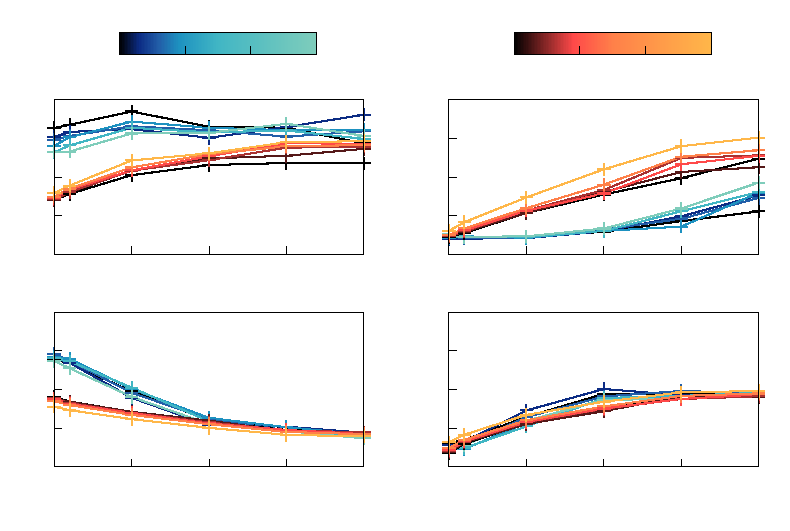
\includegraphics{licl-zif-hbonds-fit-pressure}}%
    \gplfronttext
  \end{picture}%
\endgroup

    \caption{Variations of the time constant and weights of the bi-exponential
    hydrogen bonds autocorrelation decay as function of the pressure in bulk
    (blue shades) and confined (red shades) liquids.}
    \label{fig:licl-zif:hbonds:fit:pressure}
\end{figure}

In the bulk liquid, the shortest lifetime is almost constant as the
concentration increases, but the weight of this fast process ($A_1$) decreases.
This suggests that this fastest lifetime is associated with hydrogen bonds
between water molecules surrounded only by other water molecules. As more and
more ions are added in the system, water molecules are less likely to be
surrounded only by other water molecules --- as is indicated by the results we
presented in section~\ref{sec:liquid-structure}. We also note that this
lifetime is smaller in the confined liquid than it is in the bulk phase, which
has already been shown for water at interfaces:
\citeauthor{Fogarty2014}\cite{Fogarty2014} showed that it is linked to the
librational motions of the OH bonds, and the dynamics of these "dangling" OH
groups at interfaces is faster than bulk\cite{Scatena2001}. On the other hand,
the second lifetime, associated to the slowest process, increases with
concentration, as well as the corresponding weight ($A_2$). This points to
hydrogen bonds between water molecules bounded to ions.

In the confined liquid, weights still evolve in the same way with respect to the
concentration, which point to them being associated with the same kind of
hydrogen bonds. The second lifetime increases in the confined liquid compared to
the bulk liquid. This slowdown of water dynamics under confinement is
well-known\cite{Fogarty2014}, and has been observed in many classes of
nanoporous materials\cite{Jeffery2004, RomeroVargasCastrillon2009, Haigis2013,
Scalfi2018}. It is attributed to the stronger organization of water as well as
water molecules finding fewer partners for hydrogen bond exchange. The same
arguments also apply to the increase in LiCl concentration, both in the bulk and
confined liquid. This is coherent with what we see on the changes on bulk
modulus as concentration changes in table~\ref{table:bulk}.

\begin{figure}[ht]
    \centering
    % GNUPLOT: LaTeX picture with Postscript
\begingroup
  \makeatletter
  \providecommand\color[2][]{%
    \GenericError{(gnuplot) \space\space\space\@spaces}{%
      Package color not loaded in conjunction with
      terminal option `colourtext'%
    }{See the gnuplot documentation for explanation.%
    }{Either use 'blacktext' in gnuplot or load the package
      color.sty in LaTeX.}%
    \renewcommand\color[2][]{}%
  }%
  \providecommand\includegraphics[2][]{%
    \GenericError{(gnuplot) \space\space\space\@spaces}{%
      Package graphicx or graphics not loaded%
    }{See the gnuplot documentation for explanation.%
    }{The gnuplot epslatex terminal needs graphicx.sty or graphics.sty.}%
    \renewcommand\includegraphics[2][]{}%
  }%
  \providecommand\rotatebox[2]{#2}%
  \@ifundefined{ifGPcolor}{%
    \newif\ifGPcolor
    \GPcolortrue
  }{}%
  \@ifundefined{ifGPblacktext}{%
    \newif\ifGPblacktext
    \GPblacktextfalse
  }{}%
  % define a \g@addto@macro without @ in the name:
  \let\gplgaddtomacro\g@addto@macro
  % define empty templates for all commands taking text:
  \gdef\gplbacktext{}%
  \gdef\gplfronttext{}%
  \makeatother
  \ifGPblacktext
    % no textcolor at all
    \def\colorrgb#1{}%
    \def\colorgray#1{}%
  \else
    % gray or color?
    \ifGPcolor
      \def\colorrgb#1{\color[rgb]{#1}}%
      \def\colorgray#1{\color[gray]{#1}}%
      \expandafter\def\csname LTw\endcsname{\color{white}}%
      \expandafter\def\csname LTb\endcsname{\color{black}}%
      \expandafter\def\csname LTa\endcsname{\color{black}}%
      \expandafter\def\csname LT0\endcsname{\color[rgb]{1,0,0}}%
      \expandafter\def\csname LT1\endcsname{\color[rgb]{0,1,0}}%
      \expandafter\def\csname LT2\endcsname{\color[rgb]{0,0,1}}%
      \expandafter\def\csname LT3\endcsname{\color[rgb]{1,0,1}}%
      \expandafter\def\csname LT4\endcsname{\color[rgb]{0,1,1}}%
      \expandafter\def\csname LT5\endcsname{\color[rgb]{1,1,0}}%
      \expandafter\def\csname LT6\endcsname{\color[rgb]{0,0,0}}%
      \expandafter\def\csname LT7\endcsname{\color[rgb]{1,0.3,0}}%
      \expandafter\def\csname LT8\endcsname{\color[rgb]{0.5,0.5,0.5}}%
    \else
      % gray
      \def\colorrgb#1{\color{black}}%
      \def\colorgray#1{\color[gray]{#1}}%
      \expandafter\def\csname LTw\endcsname{\color{white}}%
      \expandafter\def\csname LTb\endcsname{\color{black}}%
      \expandafter\def\csname LTa\endcsname{\color{black}}%
      \expandafter\def\csname LT0\endcsname{\color{black}}%
      \expandafter\def\csname LT1\endcsname{\color{black}}%
      \expandafter\def\csname LT2\endcsname{\color{black}}%
      \expandafter\def\csname LT3\endcsname{\color{black}}%
      \expandafter\def\csname LT4\endcsname{\color{black}}%
      \expandafter\def\csname LT5\endcsname{\color{black}}%
      \expandafter\def\csname LT6\endcsname{\color{black}}%
      \expandafter\def\csname LT7\endcsname{\color{black}}%
      \expandafter\def\csname LT8\endcsname{\color{black}}%
    \fi
  \fi
    \setlength{\unitlength}{0.0500bp}%
    \ifx\gptboxheight\undefined%
      \newlength{\gptboxheight}%
      \newlength{\gptboxwidth}%
      \newsavebox{\gptboxtext}%
    \fi%
    \setlength{\fboxrule}{0.5pt}%
    \setlength{\fboxsep}{1pt}%
\begin{picture}(5660.00,5660.00)%
    \gplgaddtomacro\gplbacktext{%
      \csname LTb\endcsname%%
      \put(752,3264){\makebox(0,0)[r]{\strut{}$0$}}%
      \csname LTb\endcsname%%
      \put(752,3700){\makebox(0,0)[r]{\strut{}$0.2$}}%
      \csname LTb\endcsname%%
      \put(752,4135){\makebox(0,0)[r]{\strut{}$0.4$}}%
      \csname LTb\endcsname%%
      \put(752,4571){\makebox(0,0)[r]{\strut{}$0.6$}}%
      \csname LTb\endcsname%%
      \put(752,5006){\makebox(0,0)[r]{\strut{}$0.8$}}%
      \csname LTb\endcsname%%
      \put(752,5442){\makebox(0,0)[r]{\strut{}$1$}}%
      \csname LTb\endcsname%%
      \put(871,3047){\makebox(0,0){\strut{}$0$}}%
      \csname LTb\endcsname%%
      \put(1979,3047){\makebox(0,0){\strut{}$5$}}%
      \csname LTb\endcsname%%
      \put(3087,3047){\makebox(0,0){\strut{}$10$}}%
      \csname LTb\endcsname%%
      \put(4194,3047){\makebox(0,0){\strut{}$15$}}%
      \csname LTb\endcsname%%
      \put(5302,3047){\makebox(0,0){\strut{}$20$}}%
    }%
    \gplgaddtomacro\gplfronttext{%
      \csname LTb\endcsname%%
      \put(178,4353){\rotatebox{-270}{\makebox(0,0){\strut{}auto correlation}}}%
      \csname LTb\endcsname%%
      \put(2631,5247){\makebox(0,0)[r]{\strut{}0 mol/L}}%
      \csname LTb\endcsname%%
      \put(2631,5030){\makebox(0,0)[r]{\strut{}1 mol/L}}%
      \csname LTb\endcsname%%
      \put(2631,4813){\makebox(0,0)[r]{\strut{}5 mol/L}}%
      \csname LTb\endcsname%%
      \put(4383,5247){\makebox(0,0)[r]{\strut{}10 mol/L}}%
      \csname LTb\endcsname%%
      \put(4383,5030){\makebox(0,0)[r]{\strut{}15 mol/L}}%
      \csname LTb\endcsname%%
      \put(4383,4813){\makebox(0,0)[r]{\strut{}20 mol/L}}%
    }%
    \gplgaddtomacro\gplbacktext{%
      \csname LTb\endcsname%%
      \put(752,694){\makebox(0,0)[r]{\strut{}$0$}}%
      \csname LTb\endcsname%%
      \put(752,1078){\makebox(0,0)[r]{\strut{}$0.2$}}%
      \csname LTb\endcsname%%
      \put(752,1462){\makebox(0,0)[r]{\strut{}$0.4$}}%
      \csname LTb\endcsname%%
      \put(752,1845){\makebox(0,0)[r]{\strut{}$0.6$}}%
      \csname LTb\endcsname%%
      \put(752,2229){\makebox(0,0)[r]{\strut{}$0.8$}}%
      \csname LTb\endcsname%%
      \put(752,2613){\makebox(0,0)[r]{\strut{}$1$}}%
      \csname LTb\endcsname%%
      \put(871,477){\makebox(0,0){\strut{}$0$}}%
      \csname LTb\endcsname%%
      \put(1979,477){\makebox(0,0){\strut{}$5$}}%
      \csname LTb\endcsname%%
      \put(3087,477){\makebox(0,0){\strut{}$10$}}%
      \csname LTb\endcsname%%
      \put(4194,477){\makebox(0,0){\strut{}$15$}}%
      \csname LTb\endcsname%%
      \put(5302,477){\makebox(0,0){\strut{}$20$}}%
    }%
    \gplgaddtomacro\gplfronttext{%
      \csname LTb\endcsname%%
      \put(178,1653){\rotatebox{-270}{\makebox(0,0){\strut{}auto correlation}}}%
      \csname LTb\endcsname%%
      \put(3086,152){\makebox(0,0){\strut{}time (ps)}}%
    }%
    \gplbacktext
    \put(0,0){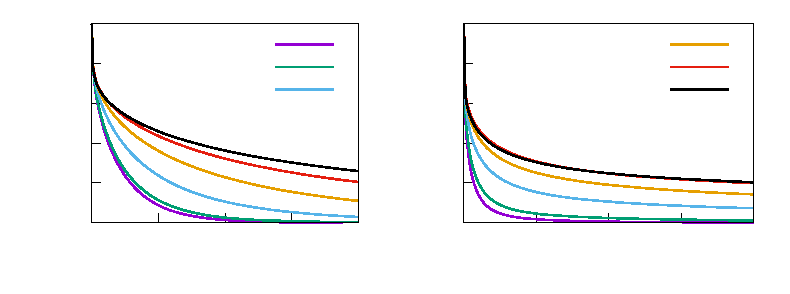
\includegraphics{licl-zif-rotcf}}%
    \gplfronttext
  \end{picture}%
\endgroup

    \caption{Rotational autocorrelation in bulk (left) and confined (right)
    electrolyte as function of LiCl concentration.}
    \label{fig:licl-zif:rotcf}
\end{figure}

\begin{table}[ht]
    \caption{Fit coefficients for the rotational autocorrelation decay from
    figure~\ref{fig:licl-zif:rotcf}.}
    \label{table:licl-zif:rotcf}
    \centering
    \renewcommand{\arraystretch}{1.3}
    \begin{tabular}{c c c c c c c c c c}
        \toprule
        \multicolumn{1}{c}{~} & \multicolumn{4}{c}{Bulk}                          &~& \multicolumn{4}{c}{Confined} \\
        \multicolumn{1}{c}{~} & $\tau_1$ (ps) & $\tau_2$ (ps) & $A_1$   & $A_2$   &~& $\tau_1$ (ps) & $\tau_2$ (ps) & $A_1$   & $A_2$   \\
        \midrule
        \SI{0}{mol/L}         &    2.69       &    1.05       & 55.6 \% & 17.2 \% &~&    0.85       &     4.65      &  32.2 \% &  5.0  \% \\
        \SI{1}{mol/L}         &    1.84       &    4.02       & 40.3 \% & 30.0 \% &~&    1.23       &     10.9      &  31.5 \% &  6.2  \% \\
        \SI{5}{mol/L}         &    2.42       &    7.69       & 33.5 \% & 37.1 \% &~&    1.92       &     24.3      &  30.6 \% &  15.9 \% \\
        \SI{10}{mol/L}        &    2.80       &    13.8       & 24.8 \% & 45.8 \% &~&    2.33       &     33.6      &  27.1 \% &  25.3 \% \\
        \SI{15}{mol/L}        &    3.24       &    22.8       & 21.4 \% & 48.5 \% &~&    2.62       &     47.1      &  24.7 \% &  30.1 \% \\
        \SI{20}{mol/L}        &    3.34       &    31.8       & 20.8 \% & 48.3 \% &~&    2.54       &     51.0      &  23.7 \% &  29.7 \% \\
        \bottomrule
    \end{tabular}
\end{table}

\begin{figure}[ht]
    \centering
    % GNUPLOT: LaTeX picture with Postscript
\begingroup
  \makeatletter
  \providecommand\color[2][]{%
    \GenericError{(gnuplot) \space\space\space\@spaces}{%
      Package color not loaded in conjunction with
      terminal option `colourtext'%
    }{See the gnuplot documentation for explanation.%
    }{Either use 'blacktext' in gnuplot or load the package
      color.sty in LaTeX.}%
    \renewcommand\color[2][]{}%
  }%
  \providecommand\includegraphics[2][]{%
    \GenericError{(gnuplot) \space\space\space\@spaces}{%
      Package graphicx or graphics not loaded%
    }{See the gnuplot documentation for explanation.%
    }{The gnuplot epslatex terminal needs graphicx.sty or graphics.sty.}%
    \renewcommand\includegraphics[2][]{}%
  }%
  \providecommand\rotatebox[2]{#2}%
  \@ifundefined{ifGPcolor}{%
    \newif\ifGPcolor
    \GPcolortrue
  }{}%
  \@ifundefined{ifGPblacktext}{%
    \newif\ifGPblacktext
    \GPblacktextfalse
  }{}%
  % define a \g@addto@macro without @ in the name:
  \let\gplgaddtomacro\g@addto@macro
  % define empty templates for all commands taking text:
  \gdef\gplbacktext{}%
  \gdef\gplfronttext{}%
  \makeatother
  \ifGPblacktext
    % no textcolor at all
    \def\colorrgb#1{}%
    \def\colorgray#1{}%
  \else
    % gray or color?
    \ifGPcolor
      \def\colorrgb#1{\color[rgb]{#1}}%
      \def\colorgray#1{\color[gray]{#1}}%
      \expandafter\def\csname LTw\endcsname{\color{white}}%
      \expandafter\def\csname LTb\endcsname{\color{black}}%
      \expandafter\def\csname LTa\endcsname{\color{black}}%
      \expandafter\def\csname LT0\endcsname{\color[rgb]{1,0,0}}%
      \expandafter\def\csname LT1\endcsname{\color[rgb]{0,1,0}}%
      \expandafter\def\csname LT2\endcsname{\color[rgb]{0,0,1}}%
      \expandafter\def\csname LT3\endcsname{\color[rgb]{1,0,1}}%
      \expandafter\def\csname LT4\endcsname{\color[rgb]{0,1,1}}%
      \expandafter\def\csname LT5\endcsname{\color[rgb]{1,1,0}}%
      \expandafter\def\csname LT6\endcsname{\color[rgb]{0,0,0}}%
      \expandafter\def\csname LT7\endcsname{\color[rgb]{1,0.3,0}}%
      \expandafter\def\csname LT8\endcsname{\color[rgb]{0.5,0.5,0.5}}%
    \else
      % gray
      \def\colorrgb#1{\color{black}}%
      \def\colorgray#1{\color[gray]{#1}}%
      \expandafter\def\csname LTw\endcsname{\color{white}}%
      \expandafter\def\csname LTb\endcsname{\color{black}}%
      \expandafter\def\csname LTa\endcsname{\color{black}}%
      \expandafter\def\csname LT0\endcsname{\color{black}}%
      \expandafter\def\csname LT1\endcsname{\color{black}}%
      \expandafter\def\csname LT2\endcsname{\color{black}}%
      \expandafter\def\csname LT3\endcsname{\color{black}}%
      \expandafter\def\csname LT4\endcsname{\color{black}}%
      \expandafter\def\csname LT5\endcsname{\color{black}}%
      \expandafter\def\csname LT6\endcsname{\color{black}}%
      \expandafter\def\csname LT7\endcsname{\color{black}}%
      \expandafter\def\csname LT8\endcsname{\color{black}}%
    \fi
  \fi
    \setlength{\unitlength}{0.0500bp}%
    \ifx\gptboxheight\undefined%
      \newlength{\gptboxheight}%
      \newlength{\gptboxwidth}%
      \newsavebox{\gptboxtext}%
    \fi%
    \setlength{\fboxrule}{0.5pt}%
    \setlength{\fboxsep}{1pt}%
\begin{picture}(7580.00,5100.00)%
    \gplgaddtomacro\gplbacktext{%
      \csname LTb\endcsname%%
      \put(408,2667){\makebox(0,0)[r]{\strut{}$0$}}%
      \csname LTb\endcsname%%
      \put(408,3037){\makebox(0,0)[r]{\strut{}$1$}}%
      \csname LTb\endcsname%%
      \put(408,3408){\makebox(0,0)[r]{\strut{}$2$}}%
      \csname LTb\endcsname%%
      \put(408,3778){\makebox(0,0)[r]{\strut{}$3$}}%
      \csname LTb\endcsname%%
      \put(408,4148){\makebox(0,0)[r]{\strut{}$4$}}%
      \csname LTb\endcsname%%
      \put(510,2481){\makebox(0,0){\strut{}$0$}}%
      \csname LTb\endcsname%%
      \put(1253,2481){\makebox(0,0){\strut{}$5$}}%
      \csname LTb\endcsname%%
      \put(1997,2481){\makebox(0,0){\strut{}$10$}}%
      \csname LTb\endcsname%%
      \put(2740,2481){\makebox(0,0){\strut{}$15$}}%
      \csname LTb\endcsname%%
      \put(3483,2481){\makebox(0,0){\strut{}$20$}}%
    }%
    \gplgaddtomacro\gplfronttext{%
      \csname LTb\endcsname%%
      \put(120,3407){\rotatebox{-270}{\makebox(0,0){\strut{}$\tau_1$ (ps)}}}%
      \csname LTb\endcsname%%
      \put(1137,4440){\makebox(0,0){\strut{}\footnotesize 0}}%
      \csname LTb\endcsname%%
      \put(1768,4440){\makebox(0,0){\strut{}\footnotesize 0.33}}%
      \csname LTb\endcsname%%
      \put(2399,4440){\makebox(0,0){\strut{}\footnotesize 0.67}}%
      \csname LTb\endcsname%%
      \put(3031,4440){\makebox(0,0){\strut{}\footnotesize 1}}%
      \csname LTb\endcsname%%
      \put(2084,5016){\makebox(0,0){\strut{}\footnotesize bulk liquid pressure (GPa)}}%
    }%
    \gplgaddtomacro\gplbacktext{%
      \csname LTb\endcsname%%
      \put(4198,2667){\makebox(0,0)[r]{\strut{}$0$}}%
      \csname LTb\endcsname%%
      \put(4198,3037){\makebox(0,0)[r]{\strut{}$25$}}%
      \csname LTb\endcsname%%
      \put(4198,3408){\makebox(0,0)[r]{\strut{}$50$}}%
      \csname LTb\endcsname%%
      \put(4198,3778){\makebox(0,0)[r]{\strut{}$75$}}%
      \csname LTb\endcsname%%
      \put(4198,4148){\makebox(0,0)[r]{\strut{}$100$}}%
      \csname LTb\endcsname%%
      \put(4300,2481){\makebox(0,0){\strut{}$0$}}%
      \csname LTb\endcsname%%
      \put(5043,2481){\makebox(0,0){\strut{}$5$}}%
      \csname LTb\endcsname%%
      \put(5787,2481){\makebox(0,0){\strut{}$10$}}%
      \csname LTb\endcsname%%
      \put(6530,2481){\makebox(0,0){\strut{}$15$}}%
      \csname LTb\endcsname%%
      \put(7273,2481){\makebox(0,0){\strut{}$20$}}%
    }%
    \gplgaddtomacro\gplfronttext{%
      \csname LTb\endcsname%%
      \put(3808,3407){\rotatebox{-270}{\makebox(0,0){\strut{}$\tau_2$ (ps)}}}%
    }%
    \gplgaddtomacro\gplbacktext{%
      \csname LTb\endcsname%%
      \put(408,627){\makebox(0,0)[r]{\strut{}$0$}}%
      \csname LTb\endcsname%%
      \put(408,998){\makebox(0,0)[r]{\strut{}$25$}}%
      \csname LTb\endcsname%%
      \put(408,1368){\makebox(0,0)[r]{\strut{}$50$}}%
      \csname LTb\endcsname%%
      \put(408,1739){\makebox(0,0)[r]{\strut{}$75$}}%
      \csname LTb\endcsname%%
      \put(408,2109){\makebox(0,0)[r]{\strut{}$100$}}%
      \csname LTb\endcsname%%
      \put(510,441){\makebox(0,0){\strut{}$0$}}%
      \csname LTb\endcsname%%
      \put(1253,441){\makebox(0,0){\strut{}$5$}}%
      \csname LTb\endcsname%%
      \put(1997,441){\makebox(0,0){\strut{}$10$}}%
      \csname LTb\endcsname%%
      \put(2740,441){\makebox(0,0){\strut{}$15$}}%
      \csname LTb\endcsname%%
      \put(3483,441){\makebox(0,0){\strut{}$20$}}%
    }%
    \gplgaddtomacro\gplfronttext{%
      \csname LTb\endcsname%%
      \put(69,1368){\rotatebox{-270}{\makebox(0,0){\strut{}$A_1$ (\%)}}}%
      \csname LTb\endcsname%%
      \put(1996,162){\makebox(0,0){\strut{}\footnotesize concentration (mol/L)}}%
    }%
    \gplgaddtomacro\gplbacktext{%
      \csname LTb\endcsname%%
      \put(4198,627){\makebox(0,0)[r]{\strut{}$0$}}%
      \csname LTb\endcsname%%
      \put(4198,998){\makebox(0,0)[r]{\strut{}$25$}}%
      \csname LTb\endcsname%%
      \put(4198,1368){\makebox(0,0)[r]{\strut{}$50$}}%
      \csname LTb\endcsname%%
      \put(4198,1739){\makebox(0,0)[r]{\strut{}$75$}}%
      \csname LTb\endcsname%%
      \put(4198,2109){\makebox(0,0)[r]{\strut{}$100$}}%
      \csname LTb\endcsname%%
      \put(4300,441){\makebox(0,0){\strut{}$0$}}%
      \csname LTb\endcsname%%
      \put(5043,441){\makebox(0,0){\strut{}$5$}}%
      \csname LTb\endcsname%%
      \put(5787,441){\makebox(0,0){\strut{}$10$}}%
      \csname LTb\endcsname%%
      \put(6530,441){\makebox(0,0){\strut{}$15$}}%
      \csname LTb\endcsname%%
      \put(7273,441){\makebox(0,0){\strut{}$20$}}%
    }%
    \gplgaddtomacro\gplfronttext{%
      \csname LTb\endcsname%%
      \put(3808,1368){\rotatebox{-270}{\makebox(0,0){\strut{}$A_2$ (\%)}}}%
      \csname LTb\endcsname%%
      \put(5786,162){\makebox(0,0){\strut{}\footnotesize concentration (mol/L)}}%
    }%
    \gplgaddtomacro\gplbacktext{%
    }%
    \gplgaddtomacro\gplfronttext{%
      \csname LTb\endcsname%%
      \put(4926,4440){\makebox(0,0){\strut{}\footnotesize 0}}%
      \csname LTb\endcsname%%
      \put(5557,4440){\makebox(0,0){\strut{}\footnotesize 0.33}}%
      \csname LTb\endcsname%%
      \put(6188,4440){\makebox(0,0){\strut{}\footnotesize 0.67}}%
      \csname LTb\endcsname%%
      \put(6820,4440){\makebox(0,0){\strut{}\footnotesize 1}}%
      \csname LTb\endcsname%%
      \put(5873,5016){\makebox(0,0){\strut{}\footnotesize confined liquid pressure (GPa)}}%
    }%
    \gplgaddtomacro\gplbacktext{%
    }%
    \gplgaddtomacro\gplfronttext{%
    }%
    \gplgaddtomacro\gplbacktext{%
    }%
    \gplgaddtomacro\gplfronttext{%
    }%
    \gplgaddtomacro\gplbacktext{%
    }%
    \gplgaddtomacro\gplfronttext{%
    }%
    \gplbacktext
    \put(0,0){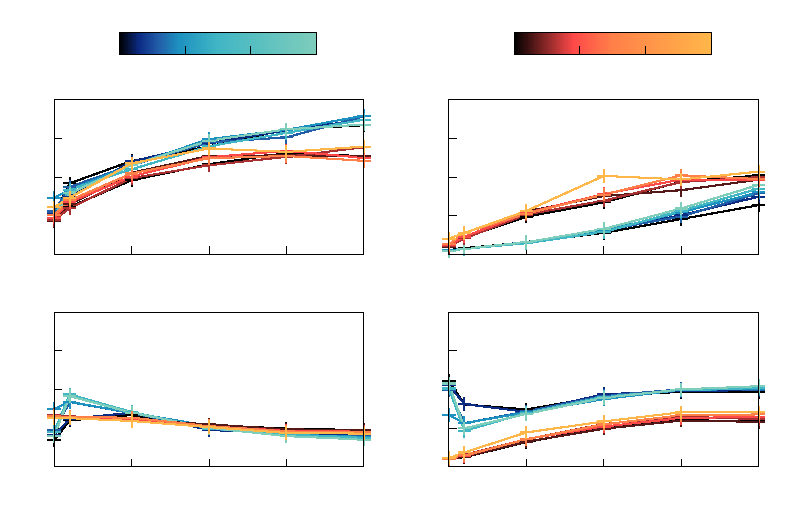
\includegraphics{licl-zif-rotcf-fit-pressure}}%
    \gplfronttext
  \end{picture}%
\endgroup

    \caption{Variations of the time constant and weights of the bi-exponential
    rotational autocorrelation decay as function of the pressure in bulk
    (blue shades) and confined (red shades) liquids.}
    \label{fig:licl-zif:rotcf:fit:pressure}
\end{figure}

\subsection{Deformation of the framework}
\label{sec:deformation}

We have studied the property of the confined liquid inside the \ZIF8 framework,
and the changes in the structure and dynamic of this liquid as it goes from a
bulk to a confined state. It is also interesting to look at the changes the
framework undergoes when going from an empty state to an intruded state.
Macroscopic changes to the volume are relatively small (less than 4\%), and
presented in the next section, specially in figure~\ref{fig:licl-zif:pv}. In this section
we will look at the internal deformations of the framework under intrusion.

Following previous works on the flexibility of \ZIF8\cite{Chaplais2018,
Coudert2017, FairenJimenez2011}, we used the distribution of the
\ce{Zn-Zn-Zn-CH3} dihedral angle (also called swing angle) to characterize the
deformations of the framework under intrusion. This angle describe the rotation
of the methyl-imidazolate linker around the surrounding zincs axis. The
distributions for empty and intruded \ZIF8 are presented in
figure~\ref{fig:licl-zif:dihedrals}.

\begin{figure}[ht]
    \centering
    % GNUPLOT: LaTeX picture with Postscript
\begingroup
  \makeatletter
  \providecommand\color[2][]{%
    \GenericError{(gnuplot) \space\space\space\@spaces}{%
      Package color not loaded in conjunction with
      terminal option `colourtext'%
    }{See the gnuplot documentation for explanation.%
    }{Either use 'blacktext' in gnuplot or load the package
      color.sty in LaTeX.}%
    \renewcommand\color[2][]{}%
  }%
  \providecommand\includegraphics[2][]{%
    \GenericError{(gnuplot) \space\space\space\@spaces}{%
      Package graphicx or graphics not loaded%
    }{See the gnuplot documentation for explanation.%
    }{The gnuplot epslatex terminal needs graphicx.sty or graphics.sty.}%
    \renewcommand\includegraphics[2][]{}%
  }%
  \providecommand\rotatebox[2]{#2}%
  \@ifundefined{ifGPcolor}{%
    \newif\ifGPcolor
    \GPcolortrue
  }{}%
  \@ifundefined{ifGPblacktext}{%
    \newif\ifGPblacktext
    \GPblacktextfalse
  }{}%
  % define a \g@addto@macro without @ in the name:
  \let\gplgaddtomacro\g@addto@macro
  % define empty templates for all commands taking text:
  \gdef\gplbacktext{}%
  \gdef\gplfronttext{}%
  \makeatother
  \ifGPblacktext
    % no textcolor at all
    \def\colorrgb#1{}%
    \def\colorgray#1{}%
  \else
    % gray or color?
    \ifGPcolor
      \def\colorrgb#1{\color[rgb]{#1}}%
      \def\colorgray#1{\color[gray]{#1}}%
      \expandafter\def\csname LTw\endcsname{\color{white}}%
      \expandafter\def\csname LTb\endcsname{\color{black}}%
      \expandafter\def\csname LTa\endcsname{\color{black}}%
      \expandafter\def\csname LT0\endcsname{\color[rgb]{1,0,0}}%
      \expandafter\def\csname LT1\endcsname{\color[rgb]{0,1,0}}%
      \expandafter\def\csname LT2\endcsname{\color[rgb]{0,0,1}}%
      \expandafter\def\csname LT3\endcsname{\color[rgb]{1,0,1}}%
      \expandafter\def\csname LT4\endcsname{\color[rgb]{0,1,1}}%
      \expandafter\def\csname LT5\endcsname{\color[rgb]{1,1,0}}%
      \expandafter\def\csname LT6\endcsname{\color[rgb]{0,0,0}}%
      \expandafter\def\csname LT7\endcsname{\color[rgb]{1,0.3,0}}%
      \expandafter\def\csname LT8\endcsname{\color[rgb]{0.5,0.5,0.5}}%
    \else
      % gray
      \def\colorrgb#1{\color{black}}%
      \def\colorgray#1{\color[gray]{#1}}%
      \expandafter\def\csname LTw\endcsname{\color{white}}%
      \expandafter\def\csname LTb\endcsname{\color{black}}%
      \expandafter\def\csname LTa\endcsname{\color{black}}%
      \expandafter\def\csname LT0\endcsname{\color{black}}%
      \expandafter\def\csname LT1\endcsname{\color{black}}%
      \expandafter\def\csname LT2\endcsname{\color{black}}%
      \expandafter\def\csname LT3\endcsname{\color{black}}%
      \expandafter\def\csname LT4\endcsname{\color{black}}%
      \expandafter\def\csname LT5\endcsname{\color{black}}%
      \expandafter\def\csname LT6\endcsname{\color{black}}%
      \expandafter\def\csname LT7\endcsname{\color{black}}%
      \expandafter\def\csname LT8\endcsname{\color{black}}%
    \fi
  \fi
    \setlength{\unitlength}{0.0500bp}%
    \ifx\gptboxheight\undefined%
      \newlength{\gptboxheight}%
      \newlength{\gptboxwidth}%
      \newsavebox{\gptboxtext}%
    \fi%
    \setlength{\fboxrule}{0.5pt}%
    \setlength{\fboxsep}{1pt}%
\begin{picture}(5660.00,3400.00)%
    \gplgaddtomacro\gplbacktext{%
      \csname LTb\endcsname%%
      \put(297,477){\makebox(0,0){\strut{}$0$}}%
      \csname LTb\endcsname%%
      \put(1298,477){\makebox(0,0){\strut{}$10$}}%
      \csname LTb\endcsname%%
      \put(2299,477){\makebox(0,0){\strut{}$20$}}%
      \csname LTb\endcsname%%
      \put(3300,477){\makebox(0,0){\strut{}$30$}}%
      \csname LTb\endcsname%%
      \put(4301,477){\makebox(0,0){\strut{}$40$}}%
      \csname LTb\endcsname%%
      \put(5302,477){\makebox(0,0){\strut{}$50$}}%
    }%
    \gplgaddtomacro\gplfronttext{%
      \csname LTb\endcsname%%
      \put(2799,152){\makebox(0,0){\strut{}$\phi$ (°)}}%
      \csname LTb\endcsname%%
      \put(4383,2987){\makebox(0,0)[r]{\strut{}0 mol/L}}%
      \csname LTb\endcsname%%
      \put(4383,2770){\makebox(0,0)[r]{\strut{}1 mol/L}}%
      \csname LTb\endcsname%%
      \put(4383,2553){\makebox(0,0)[r]{\strut{}5 mol/L}}%
      \csname LTb\endcsname%%
      \put(4383,2336){\makebox(0,0)[r]{\strut{}10 mol/L}}%
      \csname LTb\endcsname%%
      \put(4383,2119){\makebox(0,0)[r]{\strut{}15 mol/L}}%
      \csname LTb\endcsname%%
      \put(4383,1902){\makebox(0,0)[r]{\strut{}20 mol/L}}%
      \csname LTb\endcsname%%
      \put(4383,1685){\makebox(0,0)[r]{\strut{}empty}}%
    }%
    \gplbacktext
    \put(0,0){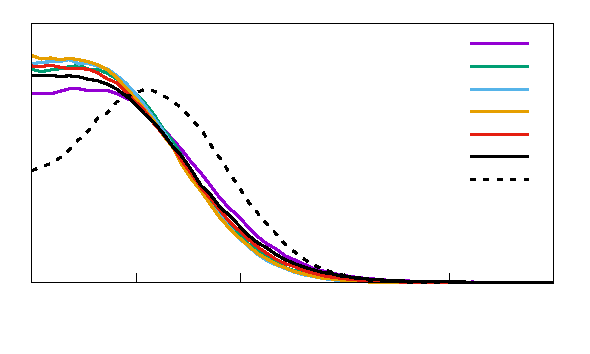
\includegraphics{licl-zif-dihedrals}}%
    \gplfronttext
  \end{picture}%
\endgroup

    \caption{Swing dihedral angle distribution in empty and intruded \ZIF8 at
    all the LiCl concentrations.}
    \label{fig:licl-zif:dihedrals}
\end{figure}

The distribution for the empty framework reproduces the already published
results: it is a Gaussian distribution, centered around the equilibrium value of
15°, and with fluctuations of the order of 10°. The distributions for \ZIF8
containing the electrolyte liquid does not seems to depend on the electrolyte
concentration. Instead they are all centered around 5°, and still have the same
order of magnitude for fluctuations. This is to be contrasted with the effect of
nitrogen adsorption at \SI{77}{K} in \ZIF8\cite{Chaplais2018}; where the
equilibrium value goes from 10° to 25° as the pores fill up with nitrogen. It is
however interesting to note that the presence of ions does not impact the
structure more than the presence of pure water does. This is coherent with the
results presented in figure~\ref{fig:licl-zif:density}, where the water molecules are
located inside the 6-member windows. Water molecules take the place of linkers
that rotate to accommodate them in the windows. As ions never enter this window,
they don't have any effect on the linkers rotation.

\subsection{Elastic properties}

Given its potential applications in mechanical energy storage, one of the most
important properties of the \ZIF8/electrolyte system is its mechanical behavior,
and notably its stability under high pressure. As an increasing stress is
applied to a material, it will first deform in a reversible and linear fashion,
in what is called the linear elastic regime. Under higher stress, the
material will start to deform in an irreversible way, and finally break.
Information on the linear elastic regime and its extent is useful to study the
stability of materials under stress, as stiffer materials are generally tougher
and able to bear higher stress before failing. This is particularly important
for soft nanoporous materials, where the mechanical stability range is lower
than in inorganic porous materials such as zeolites, and where pressure-induced
amorphization is common at moderate (sub-gigapascal)
pressures\cite{Bennett2011, Cao2012, AOrtiz2013}.

We probed the mechanical response of the \ZIF8/electrolyte system using direct
simulations of the system under explicit hydrostatic stress. We first note that
even though we allowed arbitrary changes to the unit cell lengths and tilt
factors, all the simulations cells remained orthorhombic. The figure~\ref{fig:licl-zif:pv}
present the changes in volume as the pressure increases, for all the liquid
concentrations. We can see that up to \SI{1}{GPa}, the deformation remains in
the elastic regime, and that the response is almost linear. Moreover, confining
an electrolyte in the \ZIF8 structure do not drastically affect the mechanical
properties of the system.

\begin{figure}[ht]
    \centering
    % GNUPLOT: LaTeX picture with Postscript
\begingroup
  \makeatletter
  \providecommand\color[2][]{%
    \GenericError{(gnuplot) \space\space\space\@spaces}{%
      Package color not loaded in conjunction with
      terminal option `colourtext'%
    }{See the gnuplot documentation for explanation.%
    }{Either use 'blacktext' in gnuplot or load the package
      color.sty in LaTeX.}%
    \renewcommand\color[2][]{}%
  }%
  \providecommand\includegraphics[2][]{%
    \GenericError{(gnuplot) \space\space\space\@spaces}{%
      Package graphicx or graphics not loaded%
    }{See the gnuplot documentation for explanation.%
    }{The gnuplot epslatex terminal needs graphicx.sty or graphics.sty.}%
    \renewcommand\includegraphics[2][]{}%
  }%
  \providecommand\rotatebox[2]{#2}%
  \@ifundefined{ifGPcolor}{%
    \newif\ifGPcolor
    \GPcolortrue
  }{}%
  \@ifundefined{ifGPblacktext}{%
    \newif\ifGPblacktext
    \GPblacktextfalse
  }{}%
  % define a \g@addto@macro without @ in the name:
  \let\gplgaddtomacro\g@addto@macro
  % define empty templates for all commands taking text:
  \gdef\gplbacktext{}%
  \gdef\gplfronttext{}%
  \makeatother
  \ifGPblacktext
    % no textcolor at all
    \def\colorrgb#1{}%
    \def\colorgray#1{}%
  \else
    % gray or color?
    \ifGPcolor
      \def\colorrgb#1{\color[rgb]{#1}}%
      \def\colorgray#1{\color[gray]{#1}}%
      \expandafter\def\csname LTw\endcsname{\color{white}}%
      \expandafter\def\csname LTb\endcsname{\color{black}}%
      \expandafter\def\csname LTa\endcsname{\color{black}}%
      \expandafter\def\csname LT0\endcsname{\color[rgb]{1,0,0}}%
      \expandafter\def\csname LT1\endcsname{\color[rgb]{0,1,0}}%
      \expandafter\def\csname LT2\endcsname{\color[rgb]{0,0,1}}%
      \expandafter\def\csname LT3\endcsname{\color[rgb]{1,0,1}}%
      \expandafter\def\csname LT4\endcsname{\color[rgb]{0,1,1}}%
      \expandafter\def\csname LT5\endcsname{\color[rgb]{1,1,0}}%
      \expandafter\def\csname LT6\endcsname{\color[rgb]{0,0,0}}%
      \expandafter\def\csname LT7\endcsname{\color[rgb]{1,0.3,0}}%
      \expandafter\def\csname LT8\endcsname{\color[rgb]{0.5,0.5,0.5}}%
    \else
      % gray
      \def\colorrgb#1{\color{black}}%
      \def\colorgray#1{\color[gray]{#1}}%
      \expandafter\def\csname LTw\endcsname{\color{white}}%
      \expandafter\def\csname LTb\endcsname{\color{black}}%
      \expandafter\def\csname LTa\endcsname{\color{black}}%
      \expandafter\def\csname LT0\endcsname{\color{black}}%
      \expandafter\def\csname LT1\endcsname{\color{black}}%
      \expandafter\def\csname LT2\endcsname{\color{black}}%
      \expandafter\def\csname LT3\endcsname{\color{black}}%
      \expandafter\def\csname LT4\endcsname{\color{black}}%
      \expandafter\def\csname LT5\endcsname{\color{black}}%
      \expandafter\def\csname LT6\endcsname{\color{black}}%
      \expandafter\def\csname LT7\endcsname{\color{black}}%
      \expandafter\def\csname LT8\endcsname{\color{black}}%
    \fi
  \fi
    \setlength{\unitlength}{0.0500bp}%
    \ifx\gptboxheight\undefined%
      \newlength{\gptboxheight}%
      \newlength{\gptboxwidth}%
      \newsavebox{\gptboxtext}%
    \fi%
    \setlength{\fboxrule}{0.5pt}%
    \setlength{\fboxsep}{1pt}%
\begin{picture}(5660.00,6800.00)%
    \gplgaddtomacro\gplbacktext{%
      \csname LTb\endcsname%%
      \put(595,4094){\makebox(0,0)[r]{\strut{}$15$}}%
      \csname LTb\endcsname%%
      \put(595,4716){\makebox(0,0)[r]{\strut{}$20$}}%
      \csname LTb\endcsname%%
      \put(595,5338){\makebox(0,0)[r]{\strut{}$25$}}%
      \csname LTb\endcsname%%
      \put(595,5960){\makebox(0,0)[r]{\strut{}$30$}}%
      \csname LTb\endcsname%%
      \put(595,6582){\makebox(0,0)[r]{\strut{}$35$}}%
      \csname LTb\endcsname%%
      \put(923,3877){\makebox(0,0){\strut{}$0$}}%
      \csname LTb\endcsname%%
      \put(1965,3877){\makebox(0,0){\strut{}$0.25$}}%
      \csname LTb\endcsname%%
      \put(3008,3877){\makebox(0,0){\strut{}$0.5$}}%
      \csname LTb\endcsname%%
      \put(4051,3877){\makebox(0,0){\strut{}$0.75$}}%
      \csname LTb\endcsname%%
      \put(5093,3877){\makebox(0,0){\strut{}$1$}}%
    }%
    \gplgaddtomacro\gplfronttext{%
      \csname LTb\endcsname%%
      \put(140,5338){\rotatebox{-270}{\makebox(0,0){\strut{}volume (\si{nm^3})}}}%
      \csname LTb\endcsname%%
      \put(3008,3552){\makebox(0,0){\strut{}pressure (GPa)}}%
      \csname LTb\endcsname%%
      \put(2631,6387){\makebox(0,0)[r]{\strut{}0 mol/L}}%
      \csname LTb\endcsname%%
      \put(2631,6170){\makebox(0,0)[r]{\strut{}1 mol/L}}%
      \csname LTb\endcsname%%
      \put(2631,5953){\makebox(0,0)[r]{\strut{}5 mol/L}}%
      \csname LTb\endcsname%%
      \put(4383,6387){\makebox(0,0)[r]{\strut{}10 mol/L}}%
      \csname LTb\endcsname%%
      \put(4383,6170){\makebox(0,0)[r]{\strut{}15 mol/L}}%
      \csname LTb\endcsname%%
      \put(4383,5953){\makebox(0,0)[r]{\strut{}20 mol/L}}%
    }%
    \gplgaddtomacro\gplbacktext{%
      \csname LTb\endcsname%%
      \put(595,694){\makebox(0,0)[r]{\strut{}$110$}}%
      \csname LTb\endcsname%%
      \put(595,1316){\makebox(0,0)[r]{\strut{}$120$}}%
      \csname LTb\endcsname%%
      \put(595,1939){\makebox(0,0)[r]{\strut{}$130$}}%
      \csname LTb\endcsname%%
      \put(595,2561){\makebox(0,0)[r]{\strut{}$140$}}%
      \csname LTb\endcsname%%
      \put(595,3183){\makebox(0,0)[r]{\strut{}$150$}}%
      \csname LTb\endcsname%%
      \put(923,477){\makebox(0,0){\strut{}$0$}}%
      \csname LTb\endcsname%%
      \put(1965,477){\makebox(0,0){\strut{}$0.25$}}%
      \csname LTb\endcsname%%
      \put(3008,477){\makebox(0,0){\strut{}$0.5$}}%
      \csname LTb\endcsname%%
      \put(4051,477){\makebox(0,0){\strut{}$0.75$}}%
      \csname LTb\endcsname%%
      \put(5093,477){\makebox(0,0){\strut{}$1$}}%
    }%
    \gplgaddtomacro\gplfronttext{%
      \csname LTb\endcsname%%
      \put(21,1938){\rotatebox{-270}{\makebox(0,0){\strut{}volume (\si{nm^3})}}}%
      \csname LTb\endcsname%%
      \put(3008,152){\makebox(0,0){\strut{}pressure (GPa)}}%
      \csname LTb\endcsname%%
      \put(4383,2988){\makebox(0,0)[r]{\strut{}empty}}%
    }%
    \gplbacktext
    \put(0,0){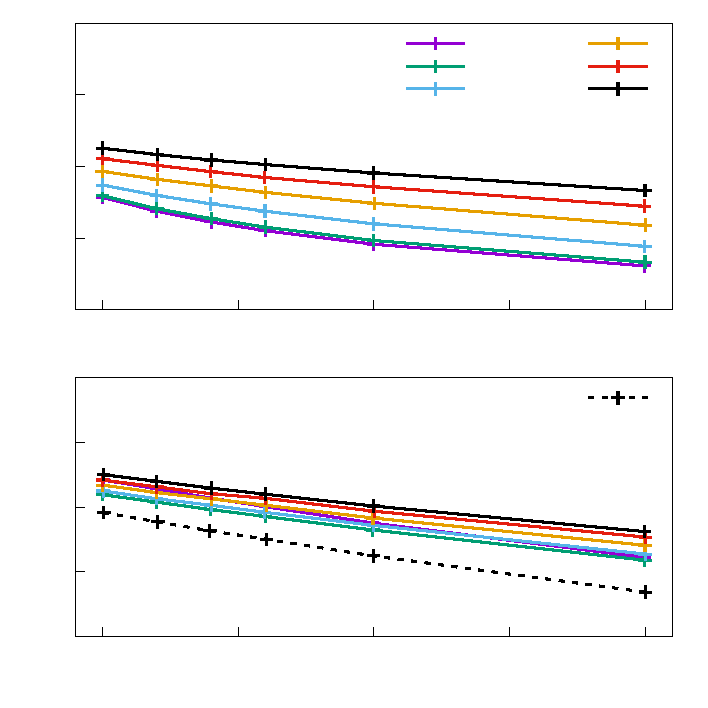
\includegraphics{licl-zif-pv}}%
    \gplfronttext
  \end{picture}%
\endgroup

    \caption{Deformation of bulk liquid (top) and \ZIF8 with confined electrolyte
    (bottom) as function of the pressure. Lines connect the different simulations
    using the same concentration.}
    \label{fig:licl-zif:pv}
\end{figure}

From these curves, we extracted the bulk modulus $K$ of the system, defined as
\[K = -V\left(\frac{\partial P}{\partial V}\right)_{N,T}\]
The values obtained in various conditions are reported in
table~\ref{table:bulk}. The value for the empty \ZIF8 is close to the
experimental\cite{Tan2012} value of \SI{7.8}{GPa}. The bulk modulii of pure
water and \SI{1}{mol/L} are further away from the experimental
values\cite{Lanman1934} of \SI{2.4}{GPa} and \SI{2.6}{GPa} respectively.
These differences are likely coming from the force-fields we used, which were
not parameterized on mechanical properties of the framework or the liquids.

\begin{table}[ht]
    \caption{Bulk modulus of the bulk electrolyte liquids and of \ZIF8
    containing a confined electrolyte liquid.}
    \label{table:bulk}
    \centering
    \renewcommand{\arraystretch}{1.5}
    \begin{tabular}{c c c}
        \toprule
        Concentration   & Bulk liquid  & Liquid $\in$ \ZIF8 \\
        \midrule
        \SI{0}{mol/L}   &    4.3 GPa   &  11.2 GPa    \\
        \SI{1}{mol/L}   &    4.4 GPa   &  13.0 GPa    \\
        \SI{5}{mol/L}   &    5.0 GPa   &  13.6 GPa    \\
        \SI{10}{mol/L}  &    6.1 GPa   &  14.4 GPa    \\
        \SI{15}{mol/L}  &    7.2 GPa   &  15.2 GPa    \\
        \SI{20}{mol/L}  &    8.4 GPa   &  15.4 GPa    \\
        \bottomrule
        Empty \ZIF8     &              &  10.5 GPa     \\
        \bottomrule
    \end{tabular}
\end{table}

The trends, however, are interesting to see. Adding water to the pores of \ZIF8
only changes the bulk modulus by a moderate amount (10\%), meaning that most of
the stiffness comes from the \ZIF8 framework --- the stiffer component of the
two. However, adding ions to the liquid has a larger effect, both in the bulk
state and the confined state, with the bulk modulus increasing by up to 50\% at
\SI{20}{mol/L} with respect to the empty framework. Since we generated the
structures in such a way that the volume occupied by the liquid is always the
same, the increase in bulk modulus is not be related to changes in the size
occupied by the ions relatively to water.  Rather, this increase in bulk modulus
comes from the stronger interactions between ions and water molecules, compared
to interactions between water molecules. The interactions between lithium
cations and water molecules are stronger than water--water hydrogen bonds, and
will make the liquid less compressible, especially at high concentration where,
statistically, all water molecules are bonded to at least one lithium atom. This
is further supported by the fact that the bulk modulus increases by the same
order of magnitude ($\approx$ \SI{5}{GPa}) in both the bulk liquid and the
confined liquid in \ZIF8.

\subsection{Thermodynamics of the intrusion}

In order to shed light into the thermodynamics of electrolyte intrusion in
\ZIF8, we extracted the potential energy for various sub-components of the total
system by taking the average value of the interaction energy of the
corresponding sub-components. The resulting average energies are presented in
table~\ref{table:thermo:raw}; where $E_\text{total}$ is the total potential
energy of the electrolyte confined in \ZIF8; $E_\text{ZIF}$ is the interaction
of \ZIF8 with itself; $E_\text{LiCl}$ is the interaction of the confined
electrolyte with itself; and $E_\text{ZIF/LiCl}$ is the interaction of the
electrolyte with the \ZIF8. $E_\text{LiCl}^\text{bulk}$ refers to the total
potential energy of the bulk electrolyte with the same number of particles as
the confined one. Every quantity is expressed for one unit cell of \ZIF8, plus
the confined liquid inside. From these values, we can extract a few
thermodynamic quantities of interest, presented in table~\ref{table:thermo}:
\[ \Delta E_\text{ZIF} (c) = E_\text{ZIF}(c) - E_\text{ZIF}^\text{empty};\]
\[ \Delta E_\text{LiCl} (c) = E_\text{LiCl}(c) - E_\text{LiCl}^\text{bulk}(c);\]
\[ \Delta H_\text{intr} (c) = E_\text{total}(c) - E_\text{LiCl}^\text{bulk}(c) - E_\text{ZIF}^\text{empty}.\]

\begin{table}[ht]
    \caption{Average interaction energy in kcal/mol per unit cell for various
    sub-systems. See the text for the definition of each sub-system.
    For reference, $k_BT$ is \SI{0.6}{kcal/mol} at \SI{300}{K}.}
    \label{table:thermo:raw}
    \centering
    \renewcommand{\arraystretch}{1.3}
    \begin{tabular}{c c c c c c}
        \toprule
        \bf LiCl       & $E_\text{Total}$ & $E_\text{ZIF}$ & $E_\text{LiCl}$ & $E_\text{LiCl/ZIF}$ & $E_\text{LiCl}^\text{bulk}$ \\
        \midrule
        Empty          &     $-746.8$       &    $-746.8$      &                 &                      &             \\
        \SI{0}{mol/L}  &     $-1617$        &    $-758.1$      &   $-703.1$        &     $-155.5$           &   $-822.9$    \\
        \SI{1}{mol/L}  &     $-1859$        &    $-739.5$      &   $-974.0$        &     $-145.8$          &   $-1080$     \\
        \SI{5}{mol/L}  &     $-2753$        &    $-738.3$      &   $-1864$         &     $-149.7$           &   $-1995$     \\
        \SI{10}{mol/L} &     $-3628$        &    $-735.5$      &   $-2744$         &     $-148.6$           &   $-2898$     \\
        \SI{15}{mol/L} &     $-4295$        &    $-732.5$      &   $-3416$         &     $-146.0$           &   $-3581$     \\
        \SI{20}{mol/L} &     $-4818$        &    $-728.4$      &   $-3949$         &     $-140.9$           &   $-4117$     \\
        \bottomrule
    \end{tabular}
\end{table}

$\Delta E_\text{ZIF}$ is the energetic change in \ZIF8 during intrusion; $\Delta
E_\text{LiCl}$ is the energetic change in the electrolyte during intrusion; and
$\Delta H_\text{intr}$ is the intrusion enthalpy, \emph{i.e.} the enthalpy
change during the \mbox{\ZIF8 + liquid $\rightarrow$ liquid $\in$
\ZIF8} process. The sign convention is taken so that all of these energies are
negative when the confined state is more stable.

\begin{table}[ht]
    \caption{Derived thermodynamic quantities in kcal/mol per unit cell. See
    the text for the definition of each quantity.}
    \label{table:thermo}
    \centering
    \renewcommand{\arraystretch}{1.3}
    \begin{tabular}{c | c c c }
        \toprule
        \bf LiCl       & $\Delta E_\text{ZIF}$ & $\Delta E_\text{LiCl}$ & $\Delta H_\text{intr}$ \\
        \midrule
        \SI{0}{mol/L}  &    $-11.3$            &    $-120$                &    $-47.3$               \\
        \SI{1}{mol/L}  &       7.3             &    $-106$                &    $-32.2$               \\
        \SI{5}{mol/L}  &       8.5             &    $-131$                &    $-11.2$               \\
        \SI{10}{mol/L} &      11.3             &    $-154$                &     16.8               \\
        \SI{15}{mol/L} &      14.3             &    $-165$                &     32.8               \\
        \SI{20}{mol/L} &      18.4             &    $-168$                &     45.8               \\
        \bottomrule
    \end{tabular}
\end{table}

We can see in table~\ref{table:thermo} that the intrusion process has a
relatively small impact on the ZIF: the energy difference between the empty and
intruded states $\Delta E_\text{ZIF}$ is in the range of tens of $kT$ (at 300~K,
$kT \approx \SI{0.6}{kcal/mol}$). The \ZIF8 framework is slightly destabilized
(energetically) in presence of the intruded liquid except at \SI{0}{mol/L},
where it is slightly stabilized. The overall effect is small compared to the two
next trends we see. We have already shown that the presence of ions have little
to no effect on the \ZIF8 structure in section~\ref{sec:deformation}.

First, the liquid is always more energetically stable in the intruded phase than
in the bulk phase ($\Delta E_\text{LiCl}$). This might seems strange as \ZIF8 is
an hydrophobic material, but the values presented only account for energetic
contributions, and do not contain entropy. Figure~\ref{fig:licl-zif:density} shows that
the entropy of the confined liquid can indeed be expected to be lower than the
entropy of the bulk liquid, because of the strong organization of the confined
fluid. As the LiCl concentration increase, the intruded phases becomes more and
more stabilized, the ions adding additional rigidity and strong interactions in
the pores network.

Secondly, we see that the energetic behavior of the whole process ($\Delta
H_\text{intr}$) is more complex: the intrusion process is energetically
favorable for low concentrations ($\leq \SI{5}{mol/L}$), and becomes unfavorable
at higher LiCl concentrations ($\geq \SI{10}{mol/L}$). The interaction between
the liquid and \ZIF8 ($E_\text{LiCl/ZIF}$ in table~\ref{table:thermo:raw}) makes
for the difference between $\Delta E_\text{ZIF} + \Delta E_\text{LiCl}$ and
$\Delta H_\text{intr}$. Even if the process is energetically favorable at low
concentrations, intrusion is not spontaneous because of the entropy contribution
to the Gibbs free energy, which makes the adsorption overall thermodynamically
unfavorable. This balance of effects, computed here from molecular simulations,
could be measured experimentally using high-pressure calorimetry, as it has been
done for the purely siliceous silicalite-1 zeolite\cite{Karbowiak2009,
Karbowiak2010}.

\subsection{Thermodynamics of ion entry into the nanopores}

\begin{figure}[t]
    \centering
    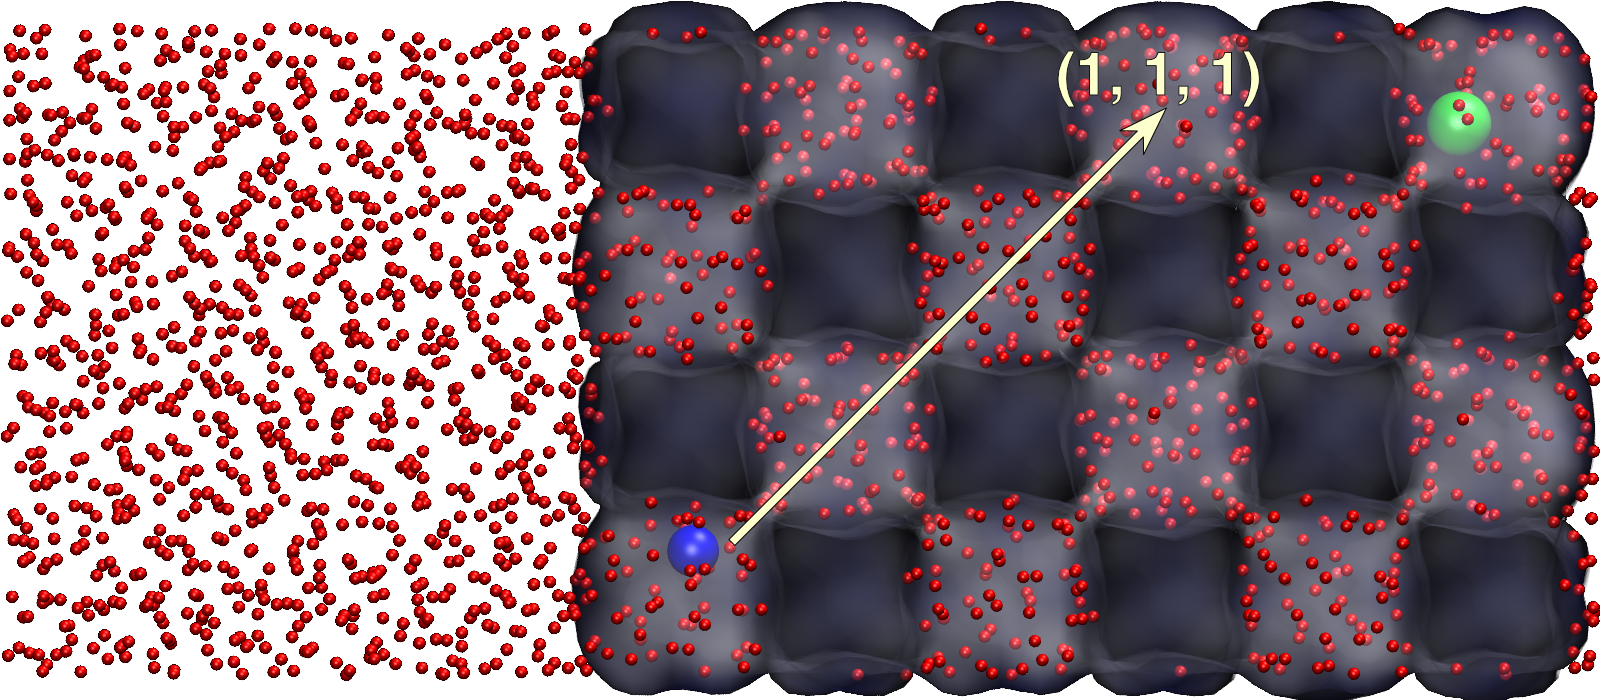
\includegraphics[width=0.9\textwidth]{figures/images/licl-zif-umbrella}
    \caption{Representation of the system used for umbrella sampling simulation
    to compute the free energy profile of entry of lithium ions in \ZIF8. We
    used similar systems for the free energy profile of entry of chlorine and
    water. Water molecules are represented in red, lithium ions in pink and
    chlorine ion in green. \ZIF8 is represented as a transparent matrix.}
    \label{fig:licl-zif:umbrella-system}
\end{figure}

In the previous sections, we described the behavior of intruded electrolytes in
the pores of \ZIF8, using full periodic boundary conditions. Here, we want to
investigate the thermodynamics of the process by which species (water molecules
and ions) can actually enter the nanopores space, \emph{i.e.} pass through the
windows of the material and its external surface. We have thus modeled an
explicit water/\ZIF8 interface, depicted in figure~\ref{fig:licl-zif:umbrella-system}:
the system here thus contains both water in the bulk state in a
\SI{34}{\angstrom}$\times$\SI{34}{\angstrom}$\times$\SI{30}{\angstrom}
reservoir, and water confined inside \ZIF8. We used the umbrella sampling
simulations and the WHAM analysis method\cite{WHAM} to reconstruct the free
energy profile of a single species (\ce{Li+}, \ce{Cl-}, or \ce{H2O}) entering
\ZIF8 along the (111) crystallographic axis. We placed the molecule of interest
at \SI{5}{\angstrom} of a window between the bulk and confined water, and the
corresponding counter ion on the other side of the \ZIF8 slab (to keep the
system neutral yet minimize ion--ion interactions). We ran a total of 121
umbrella sampling simulation for each species, spaced every
\SI{0.33}{\angstrom}. Each simulation ran for \SI{500}{ps} in the $(N, V, T)$
ensemble, using the last step of the previous simulation as starting point. The
resulting free energy profile is presented in figure~\ref{fig:licl-zif:free}, together
with the average number of neighbors at a given position on the axis (lower
panel).

\begin{figure}[ht]
    \centering
    % GNUPLOT: LaTeX picture with Postscript
\begingroup
  \makeatletter
  \providecommand\color[2][]{%
    \GenericError{(gnuplot) \space\space\space\@spaces}{%
      Package color not loaded in conjunction with
      terminal option `colourtext'%
    }{See the gnuplot documentation for explanation.%
    }{Either use 'blacktext' in gnuplot or load the package
      color.sty in LaTeX.}%
    \renewcommand\color[2][]{}%
  }%
  \providecommand\includegraphics[2][]{%
    \GenericError{(gnuplot) \space\space\space\@spaces}{%
      Package graphicx or graphics not loaded%
    }{See the gnuplot documentation for explanation.%
    }{The gnuplot epslatex terminal needs graphicx.sty or graphics.sty.}%
    \renewcommand\includegraphics[2][]{}%
  }%
  \providecommand\rotatebox[2]{#2}%
  \@ifundefined{ifGPcolor}{%
    \newif\ifGPcolor
    \GPcolortrue
  }{}%
  \@ifundefined{ifGPblacktext}{%
    \newif\ifGPblacktext
    \GPblacktextfalse
  }{}%
  % define a \g@addto@macro without @ in the name:
  \let\gplgaddtomacro\g@addto@macro
  % define empty templates for all commands taking text:
  \gdef\gplbacktext{}%
  \gdef\gplfronttext{}%
  \makeatother
  \ifGPblacktext
    % no textcolor at all
    \def\colorrgb#1{}%
    \def\colorgray#1{}%
  \else
    % gray or color?
    \ifGPcolor
      \def\colorrgb#1{\color[rgb]{#1}}%
      \def\colorgray#1{\color[gray]{#1}}%
      \expandafter\def\csname LTw\endcsname{\color{white}}%
      \expandafter\def\csname LTb\endcsname{\color{black}}%
      \expandafter\def\csname LTa\endcsname{\color{black}}%
      \expandafter\def\csname LT0\endcsname{\color[rgb]{1,0,0}}%
      \expandafter\def\csname LT1\endcsname{\color[rgb]{0,1,0}}%
      \expandafter\def\csname LT2\endcsname{\color[rgb]{0,0,1}}%
      \expandafter\def\csname LT3\endcsname{\color[rgb]{1,0,1}}%
      \expandafter\def\csname LT4\endcsname{\color[rgb]{0,1,1}}%
      \expandafter\def\csname LT5\endcsname{\color[rgb]{1,1,0}}%
      \expandafter\def\csname LT6\endcsname{\color[rgb]{0,0,0}}%
      \expandafter\def\csname LT7\endcsname{\color[rgb]{1,0.3,0}}%
      \expandafter\def\csname LT8\endcsname{\color[rgb]{0.5,0.5,0.5}}%
    \else
      % gray
      \def\colorrgb#1{\color{black}}%
      \def\colorgray#1{\color[gray]{#1}}%
      \expandafter\def\csname LTw\endcsname{\color{white}}%
      \expandafter\def\csname LTb\endcsname{\color{black}}%
      \expandafter\def\csname LTa\endcsname{\color{black}}%
      \expandafter\def\csname LT0\endcsname{\color{black}}%
      \expandafter\def\csname LT1\endcsname{\color{black}}%
      \expandafter\def\csname LT2\endcsname{\color{black}}%
      \expandafter\def\csname LT3\endcsname{\color{black}}%
      \expandafter\def\csname LT4\endcsname{\color{black}}%
      \expandafter\def\csname LT5\endcsname{\color{black}}%
      \expandafter\def\csname LT6\endcsname{\color{black}}%
      \expandafter\def\csname LT7\endcsname{\color{black}}%
      \expandafter\def\csname LT8\endcsname{\color{black}}%
    \fi
  \fi
    \setlength{\unitlength}{0.0500bp}%
    \ifx\gptboxheight\undefined%
      \newlength{\gptboxheight}%
      \newlength{\gptboxwidth}%
      \newsavebox{\gptboxtext}%
    \fi%
    \setlength{\fboxrule}{0.5pt}%
    \setlength{\fboxsep}{1pt}%
\begin{picture}(5660.00,5660.00)%
    \gplgaddtomacro\gplbacktext{%
      \csname LTb\endcsname%%
      \put(752,3264){\makebox(0,0)[r]{\strut{}$-10$}}%
      \csname LTb\endcsname%%
      \put(752,3627){\makebox(0,0)[r]{\strut{}$0$}}%
      \csname LTb\endcsname%%
      \put(752,3990){\makebox(0,0)[r]{\strut{}$10$}}%
      \csname LTb\endcsname%%
      \put(752,4353){\makebox(0,0)[r]{\strut{}$20$}}%
      \csname LTb\endcsname%%
      \put(752,4716){\makebox(0,0)[r]{\strut{}$30$}}%
      \csname LTb\endcsname%%
      \put(752,5079){\makebox(0,0)[r]{\strut{}$40$}}%
      \csname LTb\endcsname%%
      \put(752,5442){\makebox(0,0)[r]{\strut{}$50$}}%
      \csname LTb\endcsname%%
      \put(871,3047){\makebox(0,0){\strut{}$-20$}}%
      \csname LTb\endcsname%%
      \put(1425,3047){\makebox(0,0){\strut{}$-15$}}%
      \csname LTb\endcsname%%
      \put(1979,3047){\makebox(0,0){\strut{}$-10$}}%
      \csname LTb\endcsname%%
      \put(2533,3047){\makebox(0,0){\strut{}$-5$}}%
      \csname LTb\endcsname%%
      \put(3087,3047){\makebox(0,0){\strut{}$0$}}%
      \csname LTb\endcsname%%
      \put(3640,3047){\makebox(0,0){\strut{}$5$}}%
      \csname LTb\endcsname%%
      \put(4194,3047){\makebox(0,0){\strut{}$10$}}%
      \csname LTb\endcsname%%
      \put(4748,3047){\makebox(0,0){\strut{}$15$}}%
      \csname LTb\endcsname%%
      \put(5302,3047){\makebox(0,0){\strut{}$20$}}%
    }%
    \gplgaddtomacro\gplfronttext{%
      \csname LTb\endcsname%%
      \put(178,4353){\rotatebox{-270}{\makebox(0,0){\strut{}free energy (kcal/mol)}}}%
      \csname LTb\endcsname%%
      \put(2924,5247){\makebox(0,0)[r]{\strut{}\ce{Li}}}%
      \csname LTb\endcsname%%
      \put(2924,5030){\makebox(0,0)[r]{\strut{}\ce{Cl}}}%
      \csname LTb\endcsname%%
      \put(2924,4813){\makebox(0,0)[r]{\strut{}\ce{H2O}}}%
    }%
    \gplgaddtomacro\gplbacktext{%
      \csname LTb\endcsname%%
      \put(633,694){\makebox(0,0)[r]{\strut{}$0$}}%
      \csname LTb\endcsname%%
      \put(633,1078){\makebox(0,0)[r]{\strut{}$2$}}%
      \csname LTb\endcsname%%
      \put(633,1462){\makebox(0,0)[r]{\strut{}$4$}}%
      \csname LTb\endcsname%%
      \put(633,1845){\makebox(0,0)[r]{\strut{}$6$}}%
      \csname LTb\endcsname%%
      \put(633,2229){\makebox(0,0)[r]{\strut{}$8$}}%
      \csname LTb\endcsname%%
      \put(633,2613){\makebox(0,0)[r]{\strut{}$10$}}%
      \csname LTb\endcsname%%
      \put(752,477){\makebox(0,0){\strut{}$-20$}}%
      \csname LTb\endcsname%%
      \put(1321,477){\makebox(0,0){\strut{}$-15$}}%
      \csname LTb\endcsname%%
      \put(1890,477){\makebox(0,0){\strut{}$-10$}}%
      \csname LTb\endcsname%%
      \put(2458,477){\makebox(0,0){\strut{}$-5$}}%
      \csname LTb\endcsname%%
      \put(3027,477){\makebox(0,0){\strut{}$0$}}%
      \csname LTb\endcsname%%
      \put(3596,477){\makebox(0,0){\strut{}$5$}}%
      \csname LTb\endcsname%%
      \put(4165,477){\makebox(0,0){\strut{}$10$}}%
      \csname LTb\endcsname%%
      \put(4733,477){\makebox(0,0){\strut{}$15$}}%
      \csname LTb\endcsname%%
      \put(5302,477){\makebox(0,0){\strut{}$20$}}%
    }%
    \gplgaddtomacro\gplfronttext{%
      \csname LTb\endcsname%%
      \put(178,1653){\rotatebox{-270}{\makebox(0,0){\strut{}number of neighbors}}}%
      \csname LTb\endcsname%%
      \put(3027,152){\makebox(0,0){\strut{}x ($\AA$)}}%
    }%
    \gplbacktext
    \put(0,0){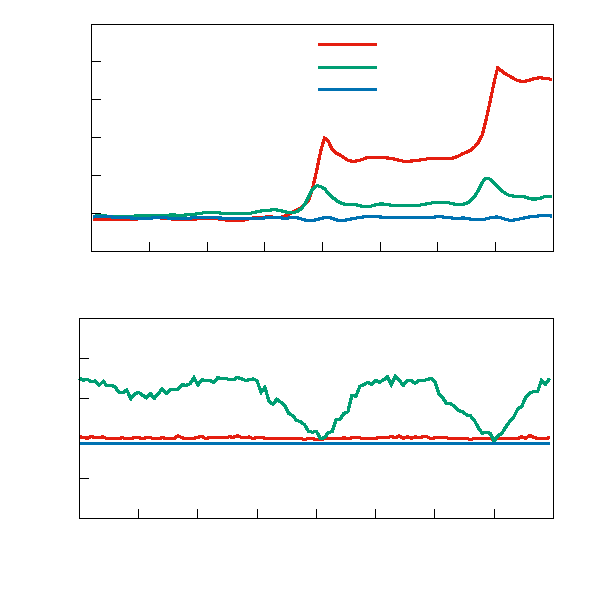
\includegraphics{licl-zif-free-energy}}%
    \gplfronttext
  \end{picture}%
\endgroup

    \caption{Free energy profile (top) of a single molecule entering \ZIF8 and
    corresponding number of neighbors (bottom) in the first solvation shell as
    function of the position of the molecule along the (111) crystallographic
    axis. The first \ZIF8 windows is at $x=0$; the $x<0$ area corresponds to
    bulk water, and the $x>0$ area to water-filled \ZIF8. We evaluated the
    uncertainty on the free energy profile using Monte Carlo
    bootstrapping\cite{WHAM}, and found it to be at most \SI{0.08}{kcal/mol} for
    \ce{H2O}, and \SI{0.3}{kcal/mol} for \ce{Cl-} and \ce{Li+}.}
    \label{fig:licl-zif:free}
\end{figure}

The first conclusion is that there is no free energy barrier for entry of the
water molecule: the energy profile is flat and the number of neighbors is
constant and around 4. This is coherent with the results already presented on
the location of water molecules inside the \ZIF8 windows and on the number of
neighbors for water molecules inside \ZIF8. It also confirms that the nature of
the liquid-phase intrusion process is not a kinetic limitation of water
adsorption, but actually due to thermodynamic hydrophobicity of the framework.
For chlorine anions, we observe two barriers on the free energy profile, which
correspond to the \ZIF8 windows at 0 and \SI{15}{\angstrom}. These barriers are
correlated to a lower number of neighbors for the anion, dropping to a value of
4: there is not enough space inside the window to fit a chlorine ion and 7 water
molecules, and the anion has to partially desolvate to pass through the window
--- explaining the presence of the free energy barrier.  Outside of these
barrier, the profile is flat and at the same level as in the bulk liquid,
meaning that while the entry of a single chlorine ion is a rare event, at long
thermodynamic time scale, Cl ions should be able to enter in \ZIF8. Generally
speaking, the Cl ions have a kinetic barrier to entry in the \ZIF8.

The results for Li are more surprising. We see both a high barrier at the first
($x=\SI{0}{\angstrom}$) and second ($x=\SI{15}{\angstrom}$) windows; and an
energetic difference between outside and inside the pores of roughly
\SI{15}{kcal/mol}. This energy difference is not only due to the bulk liquid to
confined liquid transition, as it is also present in the transition between
before and after the second window. At the same time, these barriers and energy
differences are not linked to a difference in solvation as in the chlorine case,
as the number of neighbors of lithium stays constant and around 4. Indeed, the
solvation of \ce{Li+} by water is much stronger, and its solvation sphere is
smaller in size than \ce{Cl-}. As lithium does not partially desolvate or
rearrange to pass the barrier, the whole solvation sphere needs to go though a
relatively small window, thus making the barrier higher. This points to a
difference in nature between the \ce{Li+} and \ce{Cl-} ions, which will have to
be probed further, for example by studies on other ions of different size.

\subsection{Conclusion}

Liquid intrusion of water and concentrated aqueous solutions in hydrophobic
materials have been proposed for applications in mechanical energy storage and
dissipation, and recently ZIF frameworks have been highlighted for the high
energy density that they can store. However, while the process of intrusion has
been well studied in various zeolitic materials over the last 20 years, there is
relatively little information available on the behavior --- at the microscopic
scale --- of water and electrolytes in hydrophobic metal--organic frameworks.
These systems are difficult to probe experimentally, because liquid intrusion
has to occur under high pressure. Therefore, we have used molecular dynamics
simulations to shed some light onto the properties of LiCl aqueous solutions at
various concentrations confined inside the pores of the \ZIF8 metal--organic
framework. We show that the presence of the electrolyte has a moderate impact on
the \ZIF8 framework, while the presence of the \ZIF8 matrix strongly influences
the behavior of the confined aqueous solution, affecting the overall properties
of the system. We also computed the free energy profile for the entry of water
molecules and ions into the nanopores, showing a difference between anions and
cations.

While this work provides an interesting picture of the LiCl electrolytes in
\ZIF8, it also opens a few venues for future research. The main one is the
impact of the ion size on the properties of the confined liquid. Experiments
have been performed experimentally with other ions of larger size, including
KCl, and there it is not even clear what fraction of the larger cations
(\ce{K+}) actually can diffuse inside the nanopores. Computational approaches to
these systems will be of great help in rationalizing the experimental results
and provide a view of the microscopic mechanisms that are behind them.

Another one is to give a deeper look at the free energy barriers for ions
passing through the windows of \ZIF8. While the windows are found, in the gas
phase, to be very flexible and let diffuse molecules of large diameter (up to
butane), we find that the entry of solvated species, such as ions in water, can
be linked to a significant free energy barrier. Our free energy simulations of
this process will have to be extended to other ions, in order to probe the
influence of the size of both the ion and its solvation shell, but also to look
at the influence of electrolyte concentration on the free energy profiles.
Initial tests in this direction have shown that it should be technically
possible, but convergence in such highly constrained systems is very difficult
to achieve.

Finally, this work focused on the \ZIF8 framework, perhaps the most archetypal
of the ZIF materials. The influence of framework functionalization with various
imidazolate derivatives, which has shown to greatly impact adsorption in the gas
phase, will surely also manifest itself in the liquid-phase intrusion processes.

\newpage
\section{Adsorption of water in Imogolites}

\OnlyInSubfile{\printbibliography}

\end{document}
